%MEGA MAN X.TEX

\textit{Mega Man X} was born as a spin-off game of the classic Mega Man franchise for the Super Famicom/SNES consoles (later also for PC)  between the 1993 and the 1995~\cite{wiki:MMX}. The game takes place one hundred years after the main franchise timeline, in a world where humans and special robots capable of having feelings co-exists and where X, one of those robots, fights the evil Sigma which aims to eliminate humans in order to create a world only for robots.
\begin{figure}[htp]
	\centering
	\begin{subfigure}{0.4\linewidth}
		\centering
		
\includegraphics[width=\linewidth]{figures/X1/mmx_cover.jpeg}
	\end{subfigure}
	\begin{subfigure}{0.4\linewidth}
		\centering
		
\includegraphics[width=\linewidth]{figures/X1/mmxmh.png}
	\end{subfigure}
	\caption{Cover art for the American version of X1 and its remake.}
\end{figure}

In the year 2005 a remake of the game was done for PlayStation Portable, upgraded to a 3D graphic close to the precedent title, Mega Man X8. This game (named \textit{Maverick Hunter X }or \mhx in short) had the purpose to retell the first game's story with some minor changes such as X relationship with Mavericks and Sigma, which weren't present in the original game. Changes also affected level design, such as Light's capsule positions or Sigma stages, completely different from original ones.

\section[Main plot]{Main plot (X)}
In the year 21XX humans live peacefully with a new kind of robots: reploids. Reploids are a particular type of robots with the ability to make autonomous decisions as well as having feelings and sentiments~\cite{Xcoll1:Manual_X1}. However sometimes  a reploid's electric brain can undergo  malfunctioning making him act dangerously for nearby humans and other reploids . When this happens the reploid is labeled as ``Maverick'' and has to be stopped, in order to be repaired or disposed of, by a special organization created with the exact purpose to stop mavericks: the Maverick Hunters. Leader of the Maverick Hunters is Sigma, one of the most advanced reploid of the time. 

The situation takes a turn when Sigma himself goes maverick, declaring war against humanity and recruiting in its rank other maverick hunters, both willing to follow him or threatened by Sigma himself. In order to stop the war X, the main protagonist of the story, decides to join the fight alongside Zero, a close friend of his, on the battlefield, an highway currently under attack. There he is however stopped by Vile, an ex-hunter released by Sigma from prison, in his ride armor. Only the intervention of Zero himself, which forces Vile to flee, allows X to escape safely.
\begin{figure}[htp]
	\centering
	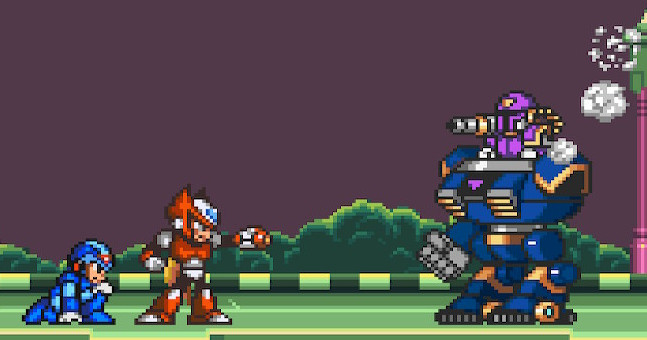
\includegraphics[width=0.5\linewidth]{figures/X1/Highway_end.jpg}
	\caption{Zero saving X from Vile.}
\end{figure}

The two then decide to split: while Zero goes to locate the enemy fortress, X has to deal with the threat of Sigma's mavericks. As X defeats all the eight mavericks, acquiring in the process new power-ups and strength, he joins Zero who in the meanwhile has located the Sigma fortress flying over the sea. At the entrance however they are immediately confronted with Vile and his ride armor, which first manages to capture Zero (that challenged him in a one-versus-one fight) and subsequently X too. As Vile laughs at his victory, Zero manages to escape from his cage, latches on the ride armor and detonates himself, destroying it but leaving Vile untouched. Seeing his friend's action gives X new energy, allowing him to break free too and face Vile, now vulnerable, defeating him in the process. Before going on however X listens to Zero's ultimate words~\cite{wiki:MMX_script}. Zero informs X that his auto-repair system cannot handle all damages taken and that X has a power even greater than his own, which makes him capable of facing Sigma (eventually Zero also gives X his own Z-buster if he didn't manage to get his own buster upgrade).

\begin{figure}[htp]
	\centering
	
\includegraphics[width=0.5\linewidth]{figures/X1/Zero_cannon.jpg}
	\caption{Zero, near death, giving X his arm cannon.}
\end{figure}
After that, Zero dies and X proceeds infiltrating Sigma's fortress and his dangers, including re-facing all the previously-defeated mavericks. At the end X arrives at Sigma's place where Sigma is waiting. At first Sigma acts with arrogance, looking surprised that X has managed to reach him with his only forces and claiming he could destroy him without effort. However he decides to leave the pleasure to his pet Velguarder, as he leaves the scene to assist at the fight. After X successfully manages to destroy Velguarder, Sigma changes his mind a little, understanding why Zero placed his trust in X and claiming X could have been a hunter as strong as he was. After that he proceeds to confront X on his own, but gets defeated and his body destroyed so that only his head remains, which subsequently proceeds to merge with a giant wolf-based mechaniloid in the room, giving Sigma a new body to fight X. However X succeeds in destroying the new body as well, effectively getting rid of Sigma for good. As Sigma blames X for destroying his dream of a world only for reploids, Sigma himself and the fortress start to explode, forcing X to teleport to the outside. In the end X ponders about the destruction he helped to generate, on the sacrifices made for the victory, and questioning if choosing to fight was the right choice, meditating if another option was possible. As the flying fortress sinks in the ocean, X realizes that he will have to fight more battles before having the answers he needs. 
After the game's credits, it is however revealed that the next battle will not take long before occurring, since a message from Sigma is played, where the maverick states that his spirit is still intact and waiting for a new body to be built to face X again.

\begin{figure}[htp]
	\centering
	
\includegraphics[width=0.45\linewidth]{figures/X1/Ending.jpg}
	
\includegraphics[width=0.45\linewidth]{figures/X1/sigma_message.jpg}
	\caption{Sigma's fortress falling in the ocean and Sigma's final message to X.}
\end{figure}

\section{Main Plot (\mhx)}
While being for the major part similar to the original plot, \textit{Maverick Hunter X} takes some divergence regarding characters relationship as well as X's background~\cite{wiki:MM_MHX}. One of the main divergence points regards X's story prior to the war's beginning. Next is a summary of \textit{Maverick Hunter X} differences respect \x.

\begin{itemize}
	\item An in-depth background of the war is given, via the ``Day of $\Sigma$"" OVA, explaining how Sigma started his revolution. Here X's background is also changed, now already being a Maverick Hunter (in contrast with the original, where no information is available) serving in the 17th Elite Unit alongside Zero and commanded by Sigma himself. X's hunter rank is B (in contrast to Zero's SA rank) due to his kindness and pacifist spirit making him prefer dialogue over fighting, traits which most mistake for weakness. The only ones suspecting of his true potential are again Zero and Sigma. 
	
	\item Another character with an expanded background is Vile. Here he aims to destroy both X and Sigma, to create his own world, hence following Sigma plans only due the fact some objectives they have match.
	
	\item A main difference between games regards the final portion of the story~\cite{wiki:MM_MHX_script} and in particular the final level's layout. In fact, while in the original X and Zero immediately face Vile as they enter Sigma fortress, here X first travels through the fortress, facing previous bosses brought back to life, and only at end he meets with Zero and is stopped by Vile. As the main story, however, Vile captures both of them, resulting in Zero sacrificing himself and X destroying him. 
	\item Finally, even Sigma has a different attitude regarding X due already suspecting X's great potential. In fact he first tests X by making him fight Velguarder (in contrast with the original game, where Sigma uses Velguarder thinking to be sufficient to defeat X) and then challenges X himself, ending in the same way as the original story.	
\end{itemize}

\section{Main Characters}
\subsection{X}
\begin{figure}[htp]
	\centering
	
\includegraphics[width=0.3\linewidth]{figures/X1/X_X1.png}
	\caption{X}
\end{figure}
X (see chap.~\ref{char:X} for full information) is the first type of a new kind of sentient robot capable of having feelings and making decisions of his own, developed by Dr. Thomas Light in the year 20XX. Being provided with great power, Dr. Light needed to ensure X's integrity by running a series of tests which would have required thirty years to be completed. Unlikely, Dr. Light's lifespan didn't allow himself to live longer to complete all tests, so he sealed X in a capsule capable of running tests in autonomy.

In the year 21XX X's capsule is found by Dr. Cain (chap. \ref{char:Cain}) during an archaeological expedition~\cite{X:Manual},~\cite{wiki:Cain_journal}. Dr. Cain awakens X and, using Light's designs and X's help, develops a new kind of robot  which he names ``Reploids'' which quickly integrates in the society due their great contribution in doing hard tasks. X however remains questioning about his place in the world and the future Dr. Light wanted for him. Despite this, when the evil Sigma starts his war against human kind, X is forced to step up and fight in order to restore peace alongside his friend Zero. 

What is told until now refers to the original role of X in the \x game. Nevertheless, as stated before, \textit{Maverick Hunter X} re-write X's story by providing a new background for events prior to Sigma's revolt. In this continuity Dr. light seals X away not for testing his integrity, but rather believing the world not to be ready for X's technology and potential. Here Light is firmly convinced that X has a good spirit and that he will use his power to achieve peace~\cite{wiki:MM_MHX_X}. Moreover after his awakening X joins the Maverick Hunters (which do not happen in the original story), serving in the 17th Elite Unit, alongside Zero and under the direct command of Sigma. Despite having great potential, however, X's hunter rank is only B (in contrast with the SA rank of Zero) due to what seems to be his lack of decision during battle. In reality this is caused by his pacifist nature, making him reluctant to fight and preventing him to use his real power~\cite{Xcoll1:Manual_X1}. Nevertheless, when the evil Sigma starts his war against human kind, X is forced to step up and fight in order to restore peace together with Zero.


\subsection{Zero}
\begin{figure}[htp]
	\centering
	
\includegraphics[width=0.3\linewidth]{figures/X1/Zero_X1.png}
	\caption{Zero}
\end{figure}
Fighting alongside X against Sigma is Zero (see chapter~\ref{char:Zero}). In the original \x game, very little information is given regarding Zero, except being a friend of X and the new leader of the Maverick Hunters~\cite{X:Manual}, having the highest rank above all hunters which didn't side with Sigma. 
Different is the situation in the \mhx game, where Zero's relationship with X is explained better, the former being a close friend and a mentor to X in the 17th Elite Unit, having an SA hunter rank and working under Sigma. Here it is also stated how Zero repels evil with all his strength, fighting merciless against Maverick, Sigma included~\cite{Xcoll1:Manual_X1}.  

In any case, Zero’s story is the same for both games. He first appears at the end of the highway saving X from Vile's grasp, and asking X to take care of Sigma forces while he locates the enemy hideout. Next he's seen at the entrance of Sigma fortress where he acts as a decoy to let X sneak inside. Lastly Zero is seen for the last time at the final battle with Vile, where he sacrifices himself to destroy Vile's armor and allow X to defeat him. Finally with his last words he asks X to go and take down Sigma, eventually giving X his own Z-buster, in case X hasn't upgraded it yet.

\section{Game Mechanics}
\textit{Mega Man X}'s gameplay stays faithful to its original series by being a 2D hybrid between a run'n'gun game and a platformer, where the main protagonist (X in this case) has to clear different stages in order to unlock the final area of the game. Each stage has its own theme, containing a certain number of items to collect (depending on the stage it could be one or more) which may require other power-ups to be collected first in order to be obtained (typically bosses weapons). Finally at the end of the stage a boss waits, which has to be defeated in order to clear the stage and which will give X a new weapon based on one of his attacks. As in the original series all main stages can be accessed in any order and all bosses presents have a ``weak point'' corresponding to a weapon obtained from defeating one another boss first. The ``weak point'' typically consists of a weapon dealing more damage to the boss, but sometimes other effects can occur, such as stunning him or preventing the boss from doing certain actions.

\x introduces however some new mechanics which will later define the series~\cite{wiki:X1_features}:
\begin{itemize}
	\item Dash: X, via the boot parts, can dash and move faster, as well as jump higher via a dash-jump. It can be considered an evolution of the sliding mechanism, as it is tied to a specific button instead of a combination of two buttons.
	\item Wall-jumping: X can jump onto walls in order to climb them or can slide down to descend slowly. He can also dash-jump off to a wall to cover a greater distance.
	\item Armor parts~[\ref{X1:Armor}]: By finding Light's capsules (four in total) X can be upgraded unlocking new powers which can help the player during the game.
	\item Sub-Weapon charging~[\ref{X1:sub_weapon}]: via the buster upgrade, X can not only charge his main X-buster, as in the main series, but he can also charge his other sub-weapon to increase damage dealt or change their functionalities.
	\item Heart tanks: beside classical Sub-tank X, eight heart tanks are also scattered in various stages (one per each). By picking them up X's energy grows by two, starting from 16 up to a maximum of 32~\cite{stratwiki:Heart_tank}.
	\item Stage interactions: although a very limited feature, by clearing certain stages, other ones will be affected and change in some portions.
\end{itemize}

\section{Weapons}\label{X1:sub_weapon}
Here is a list of all sub-weapons available in\textit{ Mega Man X}/ \textit{Mega Man Maverick Hunter X} (\cite{MHX:manual}, \cite{wiki:X_weapons}):

\subsection{
\includegraphics[width=12px, height=10px]{figures/X1/weapons/Homig_T.jpg} Homing Torpedo}\label{Homing_torpedo}
When equipping this sub-weapon, X gains the ability to fire up to two (three in \mhx)~\cite{wiki:Homing_torpedo} torpedoes capable of tracking enemies. As they pick up speed, they home in on the closest enemy and pursue it. When charged X will release a fan of four (six in \mhx) fish-shaped missiles with greater speed and attack power which home better to enemies. This weapon is obtained after defeating Launch Octopus~[\ref{boss:Launch_octopus}].
\begin{figure}[htp]
	\centering
	\begin{subfigure}{0.39\linewidth}
		
\includegraphics[width=\linewidth]{figures/X1/weapons/Homing_torpedo_1.jpg}	
	\end{subfigure}
	\begin{subfigure}{0.3\linewidth}
		
\includegraphics[width=\linewidth]{figures/X1/weapons/Homing_torpedo_2.jpg}	
	\end{subfigure}
	\caption{Homing Torpedo sub-weapon's regular and charged attack.}
\end{figure}

\subsection{
\includegraphics[width=12px, height=10px]{figures/X1/weapons/C_sting.jpg} Chameleon Sting}\label{Chameleon_sting}
The Chameleon Sting, obtained after beating Sting Chameleon ~[\ref{boss:Sting_chameleon}], emits a single straightforward laser which then splits into three directions: forward, up-forward, down-forward. In \mhx it instead directly emits three lasers, which can be angled diagonal-up and diagonal-down and are slightly faster. In both games the charged version makes X flash in various colors of the rainbow making him invincible to any damage (besides insta-kill hazards like pits) for a short amount of time. In the original game X cannot switch to any weapon while the invincibility is active, meanwhile in the remake is free to fire both with the current one and any other weapon~\cite{wiki:Chameleon_sting}.
\begin{figure}[htp]
	\centering
	\begin{subfigure}{0.35\linewidth}
		
\includegraphics[width=\linewidth]{figures/X1/weapons/Chameleon_sting.jpg}
	\end{subfigure}
	\caption{Chameleon Sting sub-weapon}
\end{figure}

\subsection{
\includegraphics[width=12px, height=10px]{figures/X1/weapons/Rolling_S.jpg} Rolling Shield}\label{Rolling_shield}
After beating Armored Armadillo ~[\ref{boss:Armored_Armadillo}], X will gain the Rolling Shield. By using it X spins energy at high speeds within the X-Buster and launches it as an energy shot that rolls along the ground. The generated projectile is about the same size as X (half in \mhx) and will roll following the ground until making contact with an enemy or disappear after a while. Only in \mhx the shield will absorb any projectile directed toward it, as well as dispose of Mets even while hiding~\cite{wiki:Rolling_shield}. Upon contact with a wall, the shield will ricochet once and disappear up hitting a wall again. When charged X will surround himself with an energy field which eliminates any enemy with less than three hit points that makes contact, but will disappear upon hitting enemies with more than that life value. In the original game while the charged shield is active X cannot shoot nor change weapon while in game, requiring the player to change weapon from the pause menu and thus making the shield disappear.
\begin{figure}[htp]
	\centering
	\begin{subfigure}{0.35\linewidth}
		
\includegraphics[width=\linewidth]{figures/X1/weapons/Rolling_shield_1.jpg}	
	\end{subfigure}
	\begin{subfigure}{0.3\linewidth}
		
\includegraphics[width=\linewidth]{figures/X1/weapons/Rolling_shield_2.jpg}	
	\end{subfigure}
	\caption{Rolling Shield sub-weapon's regular and charged attack.}
\end{figure}

\subsection{
\includegraphics[width=12px, height=10px]{figures/X1/weapons/F_wave.jpg} Fire Wave}\label{Fire_wave}
Fire Wave converts the X-buster into a powerful flamethrower, which deals continuous damage to enemies but that cannot be used underwater. Upon pressing the fire button X will start shooting fire from his X buster at a continuous rate draining energy in the process. Once charged X will fire a fireball which creates a pillar of fire upon hitting the ground and that moves forward for a while. However in order to charge the weapon X must keep firing, draining energy in the process. If used underwater the weapon won't work, only producing smoke (but still draining energy)  This weapon is obtained once Flame Mammoth is defeated~[\ref{boss:Flame_mammoth}]. 
\begin{figure}[htp]
	\centering
	\begin{subfigure}{0.35\linewidth}
		\centering
		
\includegraphics[width=\linewidth]{figures/X1/weapons/Fire_wave_1.jpg}
	\end{subfigure}
	\begin{subfigure}{0.35\linewidth}
		\centering
		
\includegraphics[width=\linewidth]{figures/X1/weapons/Fire_wave_3.jpg}
	\end{subfigure}
\end{figure}
\begin{figure}[htp]
	\ContinuedFloat
	\centering
	\begin{subfigure}{0.34\linewidth}
		\centering
		
\includegraphics[width=\linewidth]{figures/X1/weapons/Fire_wave_2.jpg}
	\end{subfigure}
	\begin{subfigure}{0.36\linewidth}
		\centering
		
\includegraphics[width=\linewidth]{figures/X1/weapons/Fire_wave_4.jpg}
	\end{subfigure}
	\caption{Fire Wave sub-weapon's regular and charged attack both outside and inside water.}
\end{figure}


\subsection{
\includegraphics[width=12px, height=10px]{figures/X1/weapons/Storm_T.jpg} Storm Tornado}\label{Storm_tornado}
The Storm Tornado turns the X-buster into a high-power fan that blasts opponents with hard-hitting wind, capable of destroying enemies that stand in its path. It shoots an horizontal tornado which stays on the screen for a short amount of time, and then starts moving in the direction X was facing when shot. Due to its length it can hit enemies multiple times, being an effective way to dispose of most of them, especially bigger ones.  The \mhx version has its length halved, which allows it to shoot at a faster rate. When charged the Storm Tornado will create a large vortex covering all the screen in high, which surrounds X in the original game while explodes instead from a shot projectile once it hits a solid surface in the remake~\cite{wiki:Storm_tornado}. It is obtained by defeating Storm Eagle~[\ref{boss:Storm_Eagle}].
\begin{figure}[htp]
	\centering
	\begin{subfigure}{0.35\linewidth}
		
\includegraphics[width=\linewidth]{figures/X1/weapons/Storm_tornado_1.jpg}
	\end{subfigure}
	\begin{subfigure}{0.25\linewidth}
		
\includegraphics[width=\linewidth]{figures/X1/weapons/Storm_tornado_2.jpg}
	\end{subfigure}
	\caption{Storm Tornado sub-weapon's regular and charged attack.}
\end{figure}

\subsection{
\includegraphics[width=12px, height=10px]{figures/X1/weapons/E_Spark.jpg} Electric Spark}\label{Electric_spark}
Electric spark creates high-pressure voltage within the X-Buster and fires it, for a maximum of three shots at time. If the electric spark hits a hard surface, it splits in half, starting to travel up and down along the surface. The charged version of this weapon differs between the original game and his remake. In X1 upon charging X will release two electric columns in front and behind him which will move in their respective directions, while in \mhx X will generate electricity in all directions from his body, covering the entire screen. This weapon is acquired upon defeating Spark Mandrill~[\ref{boss:Spark_mandrill}].
\begin{figure}[htp]
	\centering
	\begin{subfigure}{0.35\linewidth}
		
\includegraphics[width=\linewidth]{figures/X1/weapons/Electric_spark_1.jpg}
	\end{subfigure}
	\begin{subfigure}{0.25\linewidth}
		
\includegraphics[width=\linewidth]{figures/X1/weapons/Electric_spark_2.jpg}
	\end{subfigure}
	\begin{subfigure}{0.3\linewidth}
		
\includegraphics[width=\linewidth]{figures/X1/weapons/Electric_spark_3.jpg}
	\end{subfigure}
	\caption{Electric Spark sub-weapon's regular (normal and split) and charged attack.}
\end{figure}

\subsection{
\includegraphics[width=12px, height=10px]{figures/X1/weapons/B_cutter.jpg} Boomerang Cutter}\label{Boomerang_cutter}
By defeating Boomer Kuwanger~[\ref{boss:Boomer_Kuwanger}] X will gain access to the 
Boomerang Cutter. This weapon fires up to three~\cite{wiki:Boomerang_cutter} sharp boomerangs made from a special metal whose trajectory depends on the position X was when he fired them: they will arc upwards if X was standing on the ground, while they will arc downwards if X was in the air. If a boomerang does not hit an enemy, it returns to its owner, and if it passes an item on its way back, it picks up the item and delivers it to its own owner (even bringing dropped life/weapon energy from enemies). If a boomerang successfully returns to X without hitting an enemy, it will replenish the energy used to create it. Upon charging X will release four bigger boomerangs spiraling out of him diagonally. In \mhx this has been changed with four boomerangs of doubled size which will move back and forward in a straight line a few times. 

This weapon has, finally, a special perk. Both Flame Mammoth and Launch Octopus, in fact, while not being directly weak to Boomerang Cutter can be heavily damaged when hit with this weapon, the former losing his trunk and the latter his tentacles, resulting in both being unable to perform certain attacks anymore.
\begin{figure}[htp]
	\centering
	\begin{subfigure}{0.3\linewidth}
		
\includegraphics[width=\linewidth]{figures/X1/weapons/Boomerang_1.jpg}
	\end{subfigure}
	\begin{subfigure}{0.3\linewidth}
		
\includegraphics[width=\linewidth]{figures/X1/weapons/Boomerang_2.jpg}
	\end{subfigure}
	\caption{Boomerang Cutter sub-weapon's regular and charged attack.}
\end{figure}

\subsection{
\includegraphics[width=12px, height=10px]{figures/X1/weapons/S_ice.jpg} Shotgun Ice}\label{Shotgun_ice}
Shotgun Ice is the weapon obtained by X after defeating Chill Penguin ~[\ref{boss:Chill_Penguin}]. It absorbs moisture in the air and fires it in crystallized form. If it hits an enemy or a hard surface, it breaks into 5 pieces which ricochet backward and get destroyed if it hits another wall or enemy. When charged the weapon creates a Chill Penguin-shaped ice platform (only in \x, while in \mhx is only a sharp sled of ice) similar to how the boss creates his ice sculpture. X can stand on the platform which will start moving forward shortly after being created. If X creates the platform and then places himself in the same spot where the platform is creating (due the fact that the creation in not immediate) the platform will slightly push X left or right depending of its position, enabling some glitches such as wall clipping~[\ref{X1:misc}], only in \x).
\begin{figure}[htp]
	\centering
	\begin{subfigure}{0.3\linewidth}
		
\includegraphics[width=\linewidth]{figures/X1/weapons/Shotgun_ice_1.jpg}
	\end{subfigure}
	\begin{subfigure}{0.31\linewidth}
		
\includegraphics[width=\linewidth]{figures/X1/weapons/Shotgun_ice_2.jpg}
	\end{subfigure}
	\begin{subfigure}{0.29\linewidth}
		
\includegraphics[width=\linewidth]{figures/X1/weapons/Shotgun_ice_3.jpg}
	\end{subfigure}
	\caption{Shotgun Ice sub-weapon's regular (normal and deflected shots) and charged attack.}
\end{figure}

\section{First Armor}\label{X1:Armor}

While exploring stages X can run into one of the four capsules hidden by Dr.~Light. When X makes contact with the capsule, it will open revealing Dr.~Light's hologram which will talk to X and give him one of the armor parts~\cite{wiki:First_armor}, explaining in the process how it works.
\begin{figure}[htp]
	\centering
	
\includegraphics[width=0.2\linewidth]{figures/X1/First_armor.png}
	\caption{First armor X.}
\end{figure}

The First Armor is composed by the following parts:
\begin{itemize}
	\item Foot Parts:	Namely ``Emergency Acceleration System''~\cite{X:Manual} allow X to dash forward, as well as to perform dash-jumps and wall dash-jumps, also reducing his hitbox's height a little while dashing.
	\begin{figure}[htp]
		\centering
		
\includegraphics[width=0.4\textwidth]{figures/X1/Chill_penguin/Armor_foot.jpg}
		\caption{Foot Part capsule location}
	\end{figure}
	Moreover X can destroy specific blocks by wall-jumping onto them. The capsule containing the foot parts resides right in the middle of the Snow Mountain Stage, being mandatory to take. In \mhx the capsule is instead at the beginning of the Factory Stage.
	
	
	\item Body Parts: When equipped, X will have all incoming damage reduced by 50\%. It is found in the Forest stage after climbing the wall right before the cave. After defeating RT-55J the capsule will emerge from the ground. Meanwhile \textit{Maverick Hunter X} has moved it in the Storm Eagle Stage, requiring the head part to access it.
	\begin{figure}[htp]
		\centering
		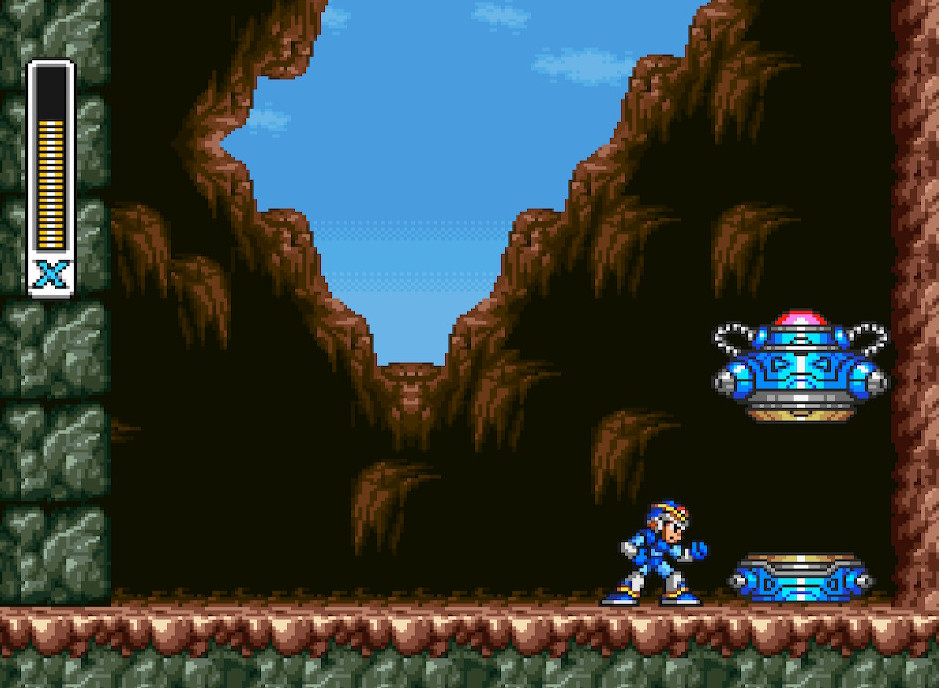
\includegraphics[width=0.4\textwidth]{figures/X1/Sting_chameleon/Sting_armor_capsule.jpg}
		\caption{Body Part capsule location}
	\end{figure}
	
	\item Arm Parts: Allow the X-Buster to be charged up to a third level, and to charge up special weapons. Originally Dr. Light thought this upgrade to be included in the basic X-Buster~\cite{X:Manual}, but he sealed away X when the upgrade was not ready yet, forcing him to turn it into a modification to give to X only later.
	\begin{figure}[htp]
		\centering
		
\includegraphics[width=0.4\textwidth]{figures/X1/Flame_mammoth/Flame_armor_2.jpg}
		\caption{Arm Parts capsule location}
	\end{figure}
	
	Despite the capsule itself not being mandatory, the game will in any case give the player the buster upgrade in form of the Z-Buster if the player arrives at facing Vile without having found the capsule first. While in \x there are no differences between the Arm Parts and the Z-Buster, in \mhx the former allow to shoot the Spiral Crush Buster, which has the same power of the second-level charged shot but is larger and hit multiple times, while the latter deals more damage against bosses that the previous alternative. In \textit{Meg Man X} the capsule resides in the Factory stage, requiring a precise dash-jump and the Head Parts to break some blocks in the ceiling, while in the remake it is in the same place the Body Parts was in the original game.
	\begin{figure}[htp]
		\centering
		
\includegraphics[width=0.5\textwidth]{figures/X1/weapons/Buster_4.jpg}
		\caption{Spiral Crush Buster attack.}
	\end{figure}
	
	
	\item Head Parts: When equipped X will gain the ability to break specific blocks with a headbutt, as well as avoid damage from falling rocks in the Forest stage (file \path{videos/X/Helmet\_protection1.mp4}). The capsule is found in the Airport stage, hidden behind an obstacle marked with a flammable warning which can be destroyed simply by shooting at it, and in Chill Penguin's stage in the remake, this time requiring the foot part to break blocks hiding it.
	\begin{figure}[htp]
		\centering
		
\includegraphics[width=0.5\textwidth]{figures/X1/Storm_eagle/Storm_armor_2.jpg}
		\caption{Head Part capsule location}
	\end{figure}
	
	\item Hadoken. While not technically being a component of the First Armor, rather a hidden bonus, this technique is stored too inside a Light's capsule so it is reported here. It allows X to perform the well-know technique from \textit{Street Fighter} by inputting the button combination $\downarrow$ $\searrow$ $\rightarrow$ (with X facing right) + fire button or using the same combination while X is charging and release the charged shot~\cite{RTA_wiki:X1}  AND X is at full health. The projectile deals 32 points of damage~\cite{wiki:Hadoken} to all enemies, basically one-shotting every non-shielded enemy, bosses included. The only exception is Sigma's final form, and only in the original \textit{Mega Man X}. 
	
	Both in the original game and its remake the capsule is hidden in Armored Armadillo Stage (see~[\ref{hadoken}] for more information on how to unlock it).
	\begin{figure}[htp]
		\centering
		\begin{subfigure}{0.3\linewidth}
			\centering
			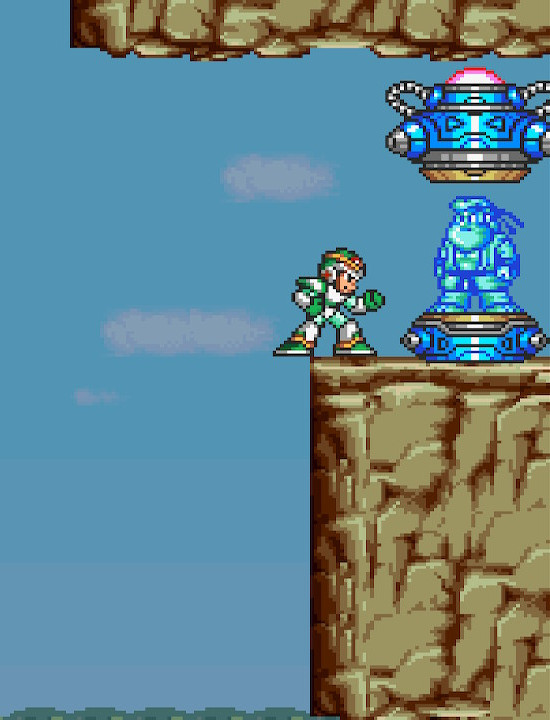
\includegraphics[width=\textwidth]{figures/X1/Armored_armadillo/Armadillo_hadoken.jpg}
		\end{subfigure}
		\begin{subfigure}{0.5\linewidth}
			\centering
			\includegraphics[width=\textwidth]{figures/X1/weapons/hadoken.jpg}
		\end{subfigure}
		\caption{hadoken Capsule location and technique}
	\end{figure}
	In any case the player has to keep in mind that, in the original game, this power-up isn't saved by the password system, meaning that it has to be re-unlocked again if the game is restarted.
\end{itemize}

\section{Highway}
The Highway Stage (Central HighWay in \textit{Maverick Hunter X}) is the first stage of the game. X arrives here in order to join the fight against Sigma's forces.
The stage is rather straightforward, having X to travel it while eliminating different enemies, and also teaching the player some basic mechanics such as wall-jumping.  The stage can be split into two main sections~\cite{stratwiki:HighWay}, the second one having more gaps and pieces of the highway falling as X stands on (recognizable by a darker texture color). In the first section of the highway two sub-bosses are presented in the form of \hyperlink{miniboss:Bee_Blader}{Bee Blader}. At the end of the stage X will be attacked by the \hyperlink{vehicle:Death_Rogumer}{Death Rogumer}, which will start sending towards him several \hyperlink{enem:Road_Attackers}{Road Attackers}.


Once some of them have been destroyed, Vile will drop out the airship and start attacking X with his ride armor. Vile is literally invincible, so there is 
no point in fighting. Instead as X drops below a certain amount of energy Vile will start shooting an energy projectile toward X and as soon as it connects, X gets trapped and the fight ends, starting the cutscene with Zero saving X. A common speedrun  technique involves having X getting hurt in order to start the boss fight with low health, which will force Vile to immediately shoot the trapping projectile and then run into it, basically skipping the entire fight.  Attention however has to be made, since Vile will not stop attacking with the armor, which may result in the player being defeated.

\begin{figure}[htp]
	\centering
	
\includegraphics[width=0.5\linewidth]{figures/X1/Highway_screenshot.jpg}
	\caption{X facing Vile.}
\end{figure}
This stage contains following enemies~\cite{wiki:Highway}:
\begin{itemize}
	\item \hyperlink{enem:Ball_De_Voux}{Ball De Voux}
	\item \hyperlink{enem:Bomb_Been}{Bomb Been}
	\item \hyperlink{enem:Crusher}{Crusher}
	\item \hyperlink{enem:Gun_Volt}{Gun Volt}
	\item \hyperlink{enem:Jamminger}{Jamminger}
	\item \hyperlink{enem:Road_Attackers}{Road Attackers}
	\item \hyperlink{enem:Spiky}{Spiky }
	\item \hyperlink{miniboss:Bee_Blader}{Bee Blader }
\end{itemize}


Once finished the introduction stage the player will be presented with the classical boss selection screen typical of the Mega Man franchise, which allows the player to choose which boss to face first. Here stages will be presented in order as they appear on the screen, from left to right, top to down.

\begin{figure}[htp]
	\centering
	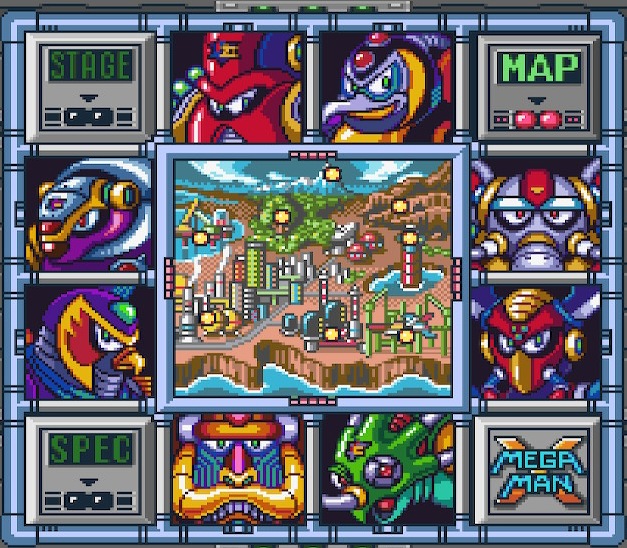
\includegraphics[width=0.5\linewidth]{figures/X1/Full_map.png}
	\caption{Full map with Bosses and their locations}
\end{figure}



\section{Ocean}
The \textit{Ocean stage} (later renamed Subterranean Base in \mhx) is where Launch Octopus hides. Here X starts from the shoreline to immerse underwater shortly after level's beginning. Once underwater X will jump higher than normal which, combined with dash-jump high reach and the beginning of the level being placed on top of a cliff, makes the player capable of skipping a good portion of stage's first part~\cite{stratwiki:Ocean}. Various fish-based enemies are present, but main difficulties come from the sub-bosses the stage has, being three plus an optional one. In the first part main difficulties are given by spiked pit which X has to jump and from where \hyperlink{enem:Sea_Attacker}{Sea Attacker} will spawn in group of three, interrupting X's jump and making him fall into the pit, and from the two \hyperlink{miniboss:Anglerge}{Anglerge} sub-bosses, the second one being particular dangerous, since the floor has two spiked pits and the Anglerge will keep using his vacuum attack to push/pull X into them. Here the best strategy consists in staying at the leftmost platform and keep shooting, dashing to the right once it starts pulling and shooting while it pushes X. Anglerges will also shoot X four serpent-shaped harpoons which will move horizontally and then fall/rise onto X when they're above/below him. Finally Anglerges will rarely shoot a beam of light from their lamp, which can be destroyed. After passing the second sub-boss the second part of the stage begins. Here spiked gaps are less common (although still present) and whirlpools will start to appear at regular intervals and in specific positions. Those whirlpools can be used to propel X up to the ocean's surface. Proceeding in the stage bombs will start dropping from above, fired by a \hyperlink{miniboss:Cruiziler}{Cruiziler} enemy. X can either climb a whirlpool to get onto it and destroy its core, making it sink and stop it from shooting bombs, or avoid it and proceed in the level. Once passed falling bombs, X will find himself in an arena filled with sand. Here an \hyperlink{miniboss:Utuboros}{Utuboros} will start attacking him, rising from the sand, then swimming for a while and then immersing again in the sand. It is invincible for most of its body (which X can stand on), only the head and tail being vulnerable. Although its weakness is considered to be the Boomerang Cutter, due to lack of invincibility frame a single Storm Tornado fired behind its head will destroy him in one shot~\cite{wiki:Utuboros}. After this other sub-boss X has to go forward only for a little before finding himself in front of the boss door.


Here is a list of all enemies present in the stage~\cite{wiki:Ocean}:
\begin{itemize}
	\item \hyperlink{enem:Amenhopper}{Amenhopper}
	\item \hyperlink{miniboss:Anglerge}{Anglerge}
	\item \hyperlink{miniboss:Cruiziler}{Cruiziler}
	\item \hyperlink{enem:Gulpfer}{Gulpfer }
	\item \hyperlink{enem:Mega_Tortoise}{Mega Tortoise }
	\item \hyperlink{enem:Sea_Attacker}{Sea Attacker}
	\item \hyperlink{enem:Sky_Claw}{Sky Claw }
	\item \hyperlink{miniboss:Utuboros}{Utuboros}
\end{itemize}

\subsection{Heart Tank}
This stage only has a heart tank. In order to get it the player must first destroy the Cruizer by reaching the ocean's surface via the closest whirlpool, climbing it and then shooting Cruizer's blue core, avoiding in the meanwhile the Sky Claws which the ship will spawn. Once destroyed, the Cruizer will sink and will destroy the ocean's floor, revealing a hidden portion with a large room filled with spiked gaps on the ground. Here another Utuboros (technically the first since the other one resides later in the level) must be defeated, in order to open the door which leads to a Heart Tank. After that X must exit from where he entered and climb the wall where the ship fell in order to return to the main path.

\begin{figure}[htp]
	\centering
	\begin{subfigure}{0.4\textwidth}
		\centering
		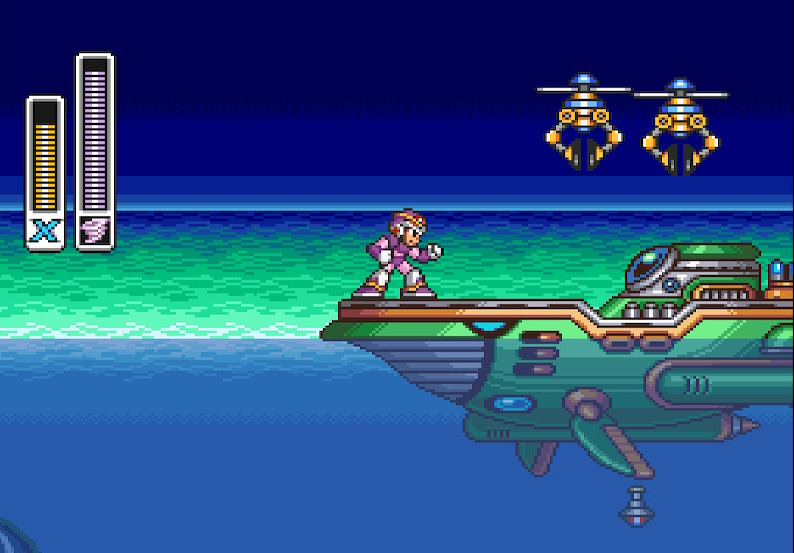
\includegraphics[height=3cm]{figures/X1/Launch_octopus/Octopus_heart_1.jpg}
		\caption{}
	\end{subfigure}
	\begin{subfigure}{0.4\textwidth}
		\centering
		
\includegraphics[height=3cm]{figures/X1/Launch_octopus/Octopus_heart_2.jpg}
		\caption{}
	\end{subfigure}\\
	\begin{subfigure}{0.4\textwidth}
		\centering
		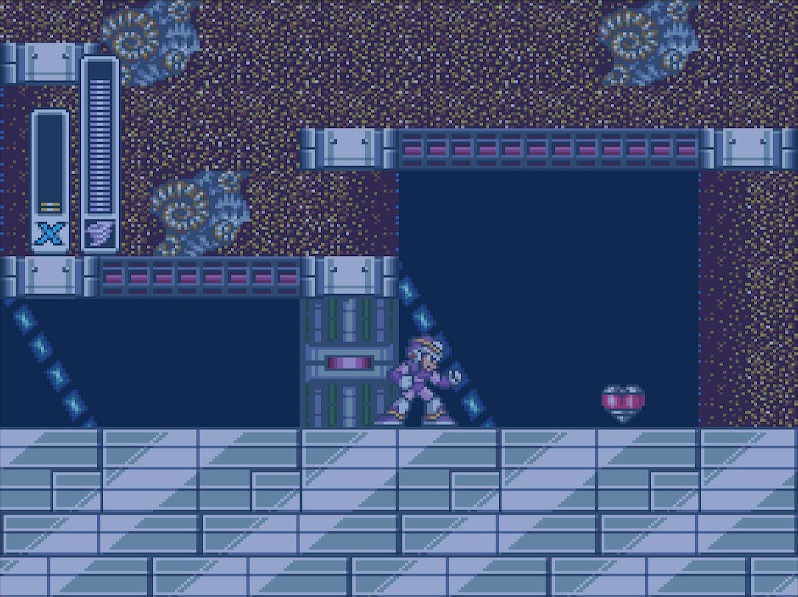
\includegraphics[height=3cm]{figures/X1/Launch_octopus/Octopus_heart_3.jpg}
		\caption{}
	\end{subfigure}
	\caption{(a)Via whirlpool the player can reach the Cruizer on ocean's surface,(b) When destroyed the ship will fall down, breaking the ocean floor and opening a new path,(c) Once destroyed the Utuboros inside the cave, a room will open with the Heart Tank inside}
\end{figure}

\subsection{Launch Octopus}\label{boss:Launch_octopus}
\begin{figure}[htp]
	\centering
	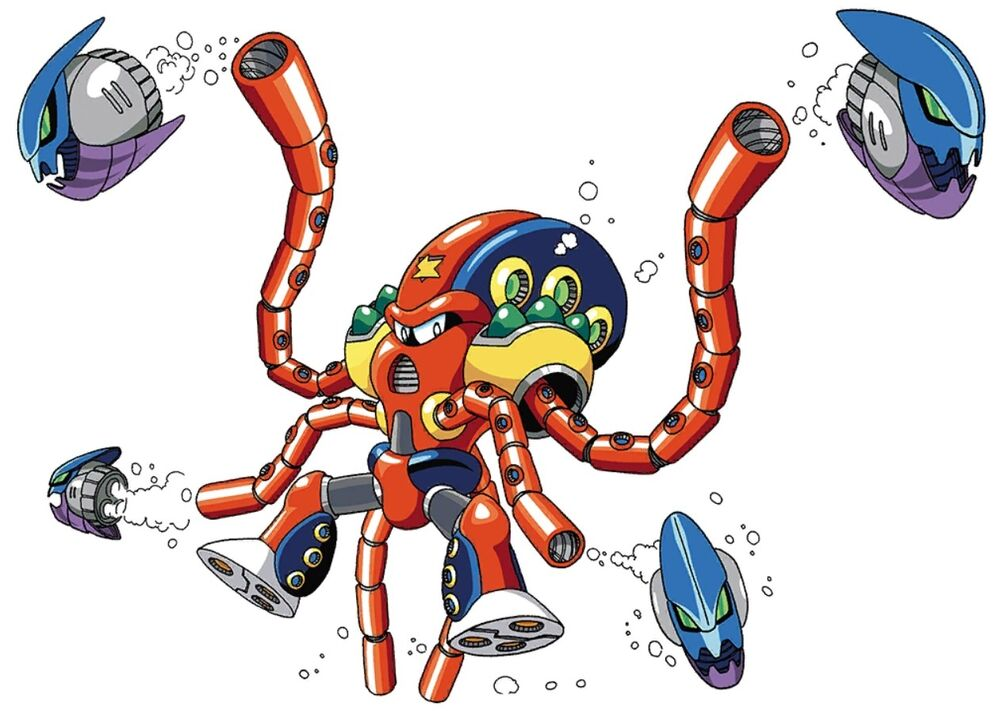
\includegraphics[height=5cm]{figures/X1/Launch_octopus/LaunchOctopus.jpg}
	
\includegraphics[height=5cm]{figures/X1/Launch_octopus/MHXLaunchOctopus.jpg}
	\caption{Launch Octopus' designs (\cite{book:MMX_Complete_art})}
\end{figure}

Launch Octopus, the ``\textit{General of the Deep Sea}''~\cite{book:MMX_Complete_art} was a Maverick Hunter of the 6th Fleet armada before joining Sigma's rebellion and setting his base in the dept of the Ocean, in order to attack marine cities with his army of mechaniloids and to cut off shipping routes. In \x he joins Sigma due the fact he shares the dream of a world only for reploids, having always doubt about protecting humans, while in \mhx he is pictured as a military tactician who wants to achieve beauty in combat, considering himself an unappreciated artist of underwater fighting. Only Sigma understood his art, making Launch Octopus side with him~\cite{wiki:MM_MHX_script}.

\begin{figure}[htp]
	\centering
	\begin{subfigure}{0.48\textwidth}
		\centering
		\includegraphics[width=\linewidth]{figures/X1/Launch_octopus/Octopus_missile.jpg}
		\caption{Homing Torpedo}
	\end{subfigure}
	\begin{subfigure}{0.49\textwidth}
		\centering
		\includegraphics[width=\linewidth]{figures/X1/Launch_octopus/Octopus_piranha.jpg}
		\caption{Charged Homing Torpedo}
	\end{subfigure}
\end{figure}

\begin{figure}
	\ContinuedFloat
	\centering
	\begin{subfigure}{0.2\textwidth}
		\centering
		\includegraphics[width=\linewidth]{figures/X1/Launch_octopus/Octopus_vortex.jpg}
		\caption{Vortex}
	\end{subfigure}
	\begin{subfigure}{0.37\textwidth}
		\centering
		\includegraphics[width=\linewidth]{figures/X1/Launch_octopus/Octopus_drain.jpg}
		\caption{Energy Drain}
	\end{subfigure}
	\begin{subfigure}{0.39\textwidth}
		\centering
		\includegraphics[width=\linewidth]{figures/X1/Launch_octopus/Octopus_cut.jpg}
		\caption{Tentacles cut off}
	\end{subfigure}
	
	\caption{Launch Octopus' attacks}
	
\end{figure}

In battle Octopus has two main techniques: Homing torpedo and Energy Drain. In reality he has a third technique, which consists in firing what can be considered a charged version of his Homing Torpedo. Both his types of missiles can be destroyed by shooting at them. Launch Octopus will always start the boss fight with a barrage of homing missiles, to then  switch to one of the other two weapons he has. Just like X, Octopus can fire a charged version of his homing missiles, which are piranha-shaped and home much faster than their counterpart. Finally he has his Energy Drain attack. When performing this Octopus will first swim on top of the arena, either left or right, and then start spinning to create a whirlpool to suck X in. If he succeeds he will start draining X energy to replenish his own, prolonging the fight until the player breaks free. Octopus main weakness is the Rolling Shield, which deals him extra damage but can be hard to hit, due Octopus high mobility and the shield colliding with his missiles instead. However Octopus can be also heavily damaged by the Boomerang Cutter, which in three hits will sever his tentacles blocking him to perform his Energy Drain attack. 


Officially~\cite{wayback:X_resources} Launch Octopus is 232 cm tall and 182 Kg heavy, in contrast with in-game information~\cite{wiki:Launch_octopus} which show a weight value smaller than actual ones (see fig ~\ref{Octopus_specs}).

Once Launch Octopus has been defeated X will gain the Homing Torpedo (\ref{Homing_torpedo}) weapon, as well as cause a flood in the Forest Stage, making water appear near the beginning of the stage.In battle Octopus has two main techniques: Homing torpedo and Energy Drain. In reality he has a third technique, which consists in firing what can be considered a charged version of his Homing Torpedo. Both his types of missiles can be destroyed by shooting at them. Launch Octopus will always start the boss fight with a barrage of homing missiles, to then  switch to one of the other two weapons he has. Just like X, Octopus can fire a charged version of his homing missiles, which are piranha-shaped and home much faster than their counterpart. Finally he has his Energy Drain attack. When performing this Octopus will first swim on top of the arena, either left or right, and then start spinning to create a whirlpool to suck X in. If he succeeds he will start draining X energy to replenish his own, prolonging the fight until the player breaks free. Octopus main weakness is the Rolling Shield, which deals him extra damage but can be hard to hit, due Octopus high mobility and the shield colliding with his missiles instead. However Octopus can be also heavily damaged by the Boomerang Cutter, which in three hits will sever his tentacles blocking him to perform his Energy Drain attack. 


Officially~\cite{wayback:X_resources} Launch Octopus is 232 cm tall and 182 Kg heavy, in contrast with in-game information~\cite{wiki:Launch_octopus} which show a weight value smaller than actual ones (see fig ~\ref{Octopus_specs}).

Once Launch Octopus has been defeated X will gain the Homing Torpedo (\ref{Homing_torpedo}) weapon, as well as cause a flood in the Forest Stage, making water appear near the beginning of the stage.


\begin{figure}[htp]
	\begin{minipage}[c]{0.45\linewidth}
		\vspace{0pt}
		\centering
		\includegraphics[width=\linewidth]{figures/X1/Launch_octopus/Launch_octopus_specs.png}
	\end{minipage}
	\begin{minipage}[c]{0.45\linewidth}
		\centering
		\vspace{0pt}
		\begin{tabular}[h]{l c}
			\toprule
			Health Bar & 32\\
			\midrule
			\multicolumn{1}{c}{Attack} & \multicolumn{1}{c}{Damage}\\
			Contact & 4\\
			Homing Torpedo & 2\\
			Charged H. Torpedo & 2\\
			Energy Drain & 1-15\\
			\bottomrule
		\end{tabular}
	\end{minipage}
	\caption{Left: Launch Octopus' specifications and according to X1; Right: In-game data~\cite{wiki:Launch_octopus}. }
	\label{Octopus_specs}
\end{figure}


\section{Snow Mountain}
\textit{Snow Mountain}(\textit{Abandoned Missile Base in \mhx}) is probably the first stage most people go when starting the game, due to its low level of danger it contains~\cite{stratwiki:Snow_mountain}, as for having inside the most useful upgrade X get can get, the Foot Parts. The stage, as the name states, takes place in a snow-covered mountain which X has to climb to get to the boss. The stage is divided into three main areas. The first area is where X starts and consists of a path that brings him inside a cave through a series of enemies. Once inside the cave (the second area) X has to climb it while avoiding enemies which drop from higher level, and then surpass some frozen platforms separated by pits until he reaches the end of the cave. In the third area X is again on the outside. Here he can take a Ride Armor and proceed for a while. With the armor X can also destroy the igloo he finds and that would otherwise start spawning enemies. Passed the first igloo a choice can be made: to keep the Ride Armor and enter the small cave which comes next, where it is request to jump some gaps using the armor while also face another enemy Ride Armor, or use the armor to reach the top of the cave (jumping out of the armor to gain extra lift), basically skipping the lower portion. After that there is a tall wall which the armor cannot surpass, forcing him to leave it behind. Here X has to follow a path full of slopes, gaps and \hyperlink{enem:Snow_Shooter}{Snow Shooters}, which will throw snowballs at him and that become bigger the longer they roll on the snowy ground. After passing these enemies, the player will reach the boss door.

The stage contains following enemies~\cite{wiki:Snow_mountain}:
\begin{itemize}
	\item \hyperlink{enem:Armor_Soldier}{Armor Soldier} (with Ride Armor)
	\item \hyperlink{enem:Axe_Max}{Axe Max}
	\item \hyperlink{enem:Batton_Bone}{Bat Bone}
	\item \hyperlink{enem:Bomb_Been}{Bomb Been}
	\item \hyperlink{enem:Flammingle}{Flammingle}
	\item \hyperlink{enem:Jamminger}{Jamminger }
	\item \hyperlink{enem:Ray_Bit}{Ray Bit}
	\item \hyperlink{enem:Snow_Shooter}{Snow Shooter}
	\item \hyperlink{enem:Spiky}{Spiky}
	\item \hyperlink{enem:Tombot}{Tombot}
\end{itemize}

\subsection{Light's Capsule}\label{X:Foot_Parts}
In Mega Man X this stage contains the Armor capsule for the Foot Parts, which allows X to dash, also allowing to perform dash-jumps and wall dash-jumps. Furthermore, dashing also reduces a little X's height and hitbox, allowing to dodge certain attacks by dashing beneath them. The capsule is found directly onto the main path after climbing the first part of the cave. Since it is right in the middle of the path it is not avoidable, making it the only mandatory capsule of the entire series.
\begin{figure}[htp]
	\centering
	\includegraphics[width=0.5\textwidth]{figures/X1/Chill_penguin/Armor_foot.jpg}
	\caption{Foot Part capsule location}
\end{figure}

In the remake \mhx, instead, this stage hides the Head Parts. The capsule is hidden in the first indoor climbing section, hidden by block breakable only via Foot Parts.

\subsection{Heart Tank}\label{Penguin:heart_tank}
The Heart Tank of this stage is hidden in the last igloo X meet before facing the section with snowballs. To reach it X has to jump using the Ride Armor. After the first igloo there is a light blue column, right before the cave with the enemy Ride Armor. From the top of the column the player has to jump with the armor and, once reached the maximum height, jump out of it in order to reach the wall which leads to the upper path. Here two other igloos are found which can be destroyed, now that the armor is gone, by using the Fire Wave weapon. In particular the last one contains the searched Heart Tank.
\begin{figure}[htp]
	\centering
	\begin{subfigure}{0.375\linewidth}
		\centering
		\includegraphics[width=\textwidth]{figures/X1/Chill_penguin/Chill_heart_1.jpg}	
		\caption{}
	\end{subfigure}
	\begin{subfigure}{0.4\linewidth}
		\centering
		\includegraphics[width=\textwidth]{figures/X1/Chill_penguin/Chill_heart_2.jpg}	
		\caption{}
	\end{subfigure}
	\caption{Heart Tank location.}
\end{figure}

\subsection{Chill Penguin}\label{boss:Chill_Penguin}
\begin{figure}[htp]
	\centering
	\includegraphics[height=5cm]{figures/X1/Chill_penguin/Chill_Penguin.jpg}
	\includegraphics[height=5cm]{figures/X1/Chill_penguin/MHXChillPenguin.jpg}
	\caption{Chill Penguin's designs (~\cite{book:MMX_Complete_art})}
\end{figure}

The ``\textit{Glacial Emperor}''~\cite{book:MMX_Complete_art}, better known as Chill Penguin was a reploid of the 13th Polar Division, specifically designed for operating in polar environments also thanks to his small-size body. However, due to the long permanence in the South Pole, away from civilization, Chill Penguin grew tired of his mission, seeking a way to get away from there. Sigma's rebellion gave him exactly what he needed to return to civilization, allowing him to escape and join Sigma in his fight. There are however some differences in how his story is told between \x and \textit{Maverick Hunter X}. In the former, after Sigma started his revolt, Chill Penguin autonomously eliminated his own commander and escaped to join Sigma~\cite{Xcoll1:Manual_X1}, seizing a mountain base in order to crush nearby cities using avalanches. Meanwhile in the remake it is Sigma himself who took Chill Penguin away from the South Pole by making him join the 17th division together with X and Zero, even before the revolution's beginning~\cite{MHX:manual}. Later, while facing X, Chill Penguin reveals that, beside leaving the South Pole, he also joined the revolt due the payment Sigma gave him~\cite{wiki:MMX_script}. Another minor difference with the original version is that, in the remake, Chill Penguin seized an abandoned missile base, suggesting his purpose was to use it to attack the cities. 

According to descriptions, Chill Penguin is known to be a belligerent, rowdy (sometimes even warped) individual, while also having trouble with his partner Flame Mammoth (\ref{boss:Flame_mammoth}) due his jealousy of Mammoth size and the latter attitude of bullying smaller reploids.


Chill Penguin is often considered the easiest boss of the game and the first one a player should face due the simplicity of avoiding his attacks, also thanks to the Foot Parts the stage gives to the player. He has four main attacks which he performs at random~\cite{wiki:Chill_Penguin}. When using his Shotgun Ice, Chill Penguin will shoot four frozen projectiles which travel in a straight line, although some of them  can fall off and slide on the ground, which shatter upon contact with a wall but can nullify X's shots if the two meet. Other times instead of his projectiles he will emit a snowy breath which will create two penguin-shaped ice sculptures and, if X is in range, will also freeze him in place. Sculptures act both as obstacles (X takes damage if he makes contact with them) and as covers since both X and Chill Penguin projectiles will be stopped by them, but can be destroyed if enough damage is dealt to them.

\begin{figure}[htp]
	\centering
	\begin{subfigure}{0.44\textwidth}
		\centering
		\includegraphics[width=\linewidth]{figures/X1/Chill_penguin/Chill_shot.jpg}
		\caption{Shotgun Ice}
	\end{subfigure}
	\begin{subfigure}{0.53\textwidth}
		\centering
		\includegraphics[width=\linewidth]{figures/X1/Chill_penguin/Chill_frozen.jpg}
		\caption{X frozen near two ice statues}
	\end{subfigure}
	\begin{subfigure}{0.5\textwidth}
		\centering
		\includegraphics[width=\linewidth]{figures/X1/Chill_penguin/Chill_shatter.jpg}
		\caption{Chill Penguin's shotgun ice stopped by his own statues}
	\end{subfigure}
	\begin{subfigure}{0.4\textwidth}
		\centering
		\includegraphics[width=\linewidth]{figures/X1/Chill_penguin/Chill_slide.jpg}
		\caption{Slide attack}
	\end{subfigure}
	\begin{subfigure}[t]{0.5\textwidth}
		\centering
		\includegraphics[width=\linewidth]{figures/X1/Chill_penguin/Chill_blizzard.jpg}
		\caption{Blizzard attack}
	\end{subfigure}
	\begin{subfigure}[t]{0.35\textwidth}
		\centering
		\includegraphics[width=\linewidth]{figures/X1/Chill_penguin/Chill_burn.jpg}
		\caption{Chill Penguin is burnt by the Fire Wave}
	\end{subfigure}
	\caption{Chill Penguin's attacks}
\end{figure}
On some occasion Chill Penguin will leap in the air and grab the hook on the ceiling, unleashing a blizzard which will push X and the statues (if present) against a wall, causing sculptures to shatter in the process. Finally he can also slide on the floor for a while, turning immediately in case he hits a wall. While in this state he is invincible, but will also get rid of the sculpture he creates.  As it is possible to see, Chill Penguins attacks only cover the low part of the arena, meaning the best strategy to fight him consists in staying on the higher part via continuous wall-jumps, only dropping to hit him when possible. Attention however must be made, since sometimes Chill Penguin will perform a high jump toward X position which can hit him even if he's  in the high corner of the room. Besides that he can be hit at any time, even when grabbing the hook, beside when sliding. Penguin’s weakness is the Fire Wave, which will burn and stun him for a while, but it has no other particular effect.

After defeating him X will gain the Shotgun Ice (\ref{Shotgun_ice}) weapon as well as freezing the lava in the Factory Stage, considerably reducing the danger level of the stage.

Chill Penguin is 163 cm tall and 108 Kg heavy, despite the information screen on the game report being different (\ref{Penguin_specs}).

\begin{figure}[htp]
	\begin{minipage}[c]{0.45\linewidth}
		\vspace{0pt}
		\centering
		\includegraphics[width=\linewidth]{figures/X1/Chill_penguin/Chill_penguin_specs.jpg}
	\end{minipage}
	\begin{minipage}[c]{0.45\linewidth}
		\centering
		\vspace{0pt}
		\begin{tabular}[h]{l c}
			\toprule
			Health Bar & 32\\
			\midrule
			\multicolumn{1}{c}{Attack} & \multicolumn{1}{c}{Damage}\\
			Contact & 6\\
			Shotgun Ice & 2\\
			Ice Breath & 0\\
			Ice statue & 4\\
			Sliding & 6\\
			\bottomrule
		\end{tabular}
	\end{minipage}
	\caption{Left: Chill Penguin's specifications and according to X1; Right: In-game data~\cite{wiki:Chill_Penguin}. }
	\label{Penguin_specs}
\end{figure}


\section{Gallery}
The Gallery Stage (or Energy Mines Ruins in \mhx) is the stage controlled by Armored Armadillo. Peculiarity of this level are its mine carts on which X can stand and, as soon as he does it, they start moving following the track, increasing their speed as they keep going and destroying all enemies that enter in contact with them. However the player must be careful, as all the carts end their run into pits, bringing X down with them if he doesn't jump off at the right moment. This stage is also famous for containing the secret Light's capsule which teaches X the hadoken technique, as well as being the best place to farm health capsules and lives.

The stage itself is rather simple. Immediately at the beginning a mine cart is present which brings the player forward in the level while also taking care of enemies until it reaches a series of gaps, one of which it cannot jump and falls into. After this sequence only a few small gaps and some enemies separate X from the next section, which begin when he has to fall off a long pit in the ground. Here as he touches the floor a \hyperlink{miniboss:Mole_Borer}{Mole Borer} will destroy the left wall and start chasing X. This enemy is invincible and its roller can insta-kill X if he touches it, so only two solutions are possible: the first one is to escape to the right, continuing in the level; the second one is, as soon as X reaches the ground, wall jump immediately to the left before the Mole Borer breaks the wall and then jump down, following it from behind (while also gaining access to the sub tank). In both cases the player has to go right to continue. The second part of the stage mirrors the first one, having again a mine cart at the beginning and another Mole Borer at the end, only this time however X will land behind it and has to follow it as it creates a passage in the mine. Finally one last cart ride takes the player through remaining enemies until it reaches an opening on the mountain and flies off over a huge gap, impossible for X to jump. Once in the air the player must jump off the cart in order to land on the other side of the pit (or grab the wall if high enough), where the boss door is.

Following enemies are present in the stage~\cite{wiki:Gallery}:

\begin{itemize}
	\item \hyperlink{enem:Batton_Bone}{Bat Bone} 
	\item \hyperlink{enem:Batton_M-501}{Batton M-501} 
	\item \hyperlink{enem:Dig_Labour}{Dig Labour} 
	\item \hyperlink{enem:Flammingle}{Flammingle} 
	\item \hyperlink{enem:Metal_Wing}{Metal Wing} 
	\item \hyperlink{enem:Metall_C-15}{Metall C-15} 
	\item \hyperlink{miniboss:Mole_Borer}{Mole Borer}
	\item \hyperlink{enem:Spiky}{Spiky}
\end{itemize}


\begin{figure}[htp]
	\centering
	\includegraphics[width=0.5\linewidth]{figures/X1/Armored_armadillo/Armadillo_tank.jpg}
	\caption{Gallery stage's subtank location}
\end{figure}

\subsection{Sub Tank}
This stage's Sub Tank is located where the first Mole Borer appears. In order to get it the player must, once arrived at the first big gap in the ground, jump into it and then immediately wall-jump to the left, in order to let the Mole Borer break the wall and go right passing under X. Once it is passed, the player can safely jump off and go left to find the sub tank where the Mole Borer originally was. 

\subsection{Heart Tank}
The heart tank is located near where the second Mole Borer is found. Once  X jumps off the gap he has to chase the mechaniloid and destroy it in time, since as it proceeds it will destroy walls which allow access to the Heart Tank. To do this the Fire Wave weapon is suggested, since it deals massive amounts of damage to it in a short amount of time. 
\begin{figure}[htp]
	\centering
	\begin{subfigure}{0.3\linewidth}
		\centering
		\includegraphics[width=\linewidth]{figures/X1/Armored_armadillo/Armadillo_heart.jpg}
		\caption{}
	\end{subfigure}
	\begin{subfigure}{0.3\textwidth}
		\centering
		\includegraphics[width=\linewidth]{figures/X1/Armored_armadillo/Armadillo_heart_2.jpg}
		\caption{}
	\end{subfigure}
	\caption{Gallery stage's heart tank location. In (a) the Mole Borer has been destroyed and X can wall jump and reach it, while in (b) the Mole Borer has passed and X cannot reach the opening anymore}
\end{figure}

\subsection{Hadoken}\label{hadoken}
The hadoken is the last upgrade X can get before facing finals stages. The capsule containing it can be unlocked only if the player has managed to collect every other upgrade in the game: eight Heart Tanks, four Sub-Tank, four armor capsules and all the weapons from bosses. Next the player has to travel through the gallery stage and reach the top of the ledge above the boss door at least three times after defeating Armored Armadillo. At the fourth time, if the player manages to reach the place at full health, near the usual health drop there will also be the secret capsule.

\begin{figure}[htp]
	\centering
	\includegraphics[width=0.3\linewidth]{figures/X1/Armored_armadillo/Armadillo_hadoken.jpg}
	\caption{hadoken capsule with Dr.Light in Ryu's attire.}
\end{figure}
The best way to make the capsule spawn is as follow: As the stage begin, the player has to travel the level (by walking or on the mine cart) unit it reaches the zone where a single \hyperlink{enem:Batton_M-501}{Batton M-501} drops from the roof (near the first Flammingle). Here the player should farm lives by continuing to kill that enemy (which has an increased drop rate for them)  and making it respawn by walking away and returning (it is suggested to use a charged Rolling Shield as it destroys it in one hit). After having accumulated enough lives (at least five) the player can proceed in the level until the last minecart is reached, making sure to be at full health by this point. Here X has first to release a charged Sting Chameleon and immediately after ride the cart until over the pit, where he should jump off and grab the ledge over the boss door, reaching the top of if. As X reaches it, he has to jump into the pit, losing a life and respawning at the last checkpoint (before the second Mole Borer). From here the player has to repeat this procedure for another three times until, at the  fourth one, the capsule will be there. In the remake the capsule does not require multiple travel through the stage, being available immediately.

Once opened the capsule will reveal Dr. Light wearing a robe similar to Ryu's one from the Street Fighter series, which will ask X to step into the capsule to teach him the technique. In the Japanese  script of the game~\cite{wordpress:X_japanese_script} Light states that he trained under the nearby waterfall a lot to learn it, and that he will now teach it to X who can learn it, as stated again by Light himself in the remake, due to him having a nearly-human soul.


\subsection{Armored Armadillo}\label{boss:Armored_Armadillo}
\begin{figure}[htp]
	\centering
	\includegraphics[height=5cm]{figures/X1/Armored_armadillo/Armored_armadillo.jpg}
	\includegraphics[height=5cm]{figures/X1/Armored_armadillo/MHXArmoredArmadillo.png}
	\caption{Armored Armadillo's designs (~\cite{book:MMX_Complete_art})}
\end{figure}
Armored Armadillo was the commander in charge of the 8th armored force, as well as a soldier loyal to his superior, Sigma. Once the latter started his revolt, Armored Armadillo blindly followed his orders, occupying a mine to extract raw materials from which Sigma aims to create weapons for his plans.

Faithful to his name and title (``\textit{Armored Warrior}''~\cite{book:MMX_Complete_art}) Armored Armadillo fights by using his impenetrable armor both as a shield to deflect X shots and as a weapon to crush him while using his main attack, the Rolling Shield, which see him turning into a ball and start bouncing off arena's walls while also being immune to any attack. On some occasions Armadillo will also take out the cannon hidden in his forehead and start shooting a sequence of rapid bullets in a straight line before beginning to roll again. 

\begin{figure}[htp]
	\centering
	\begin{subfigure}{0.45\textwidth}
		\centering
		\includegraphics[height=4cm]{figures/X1/Armored_armadillo/Armadillo_rolling.jpg}
		\caption{Rolling Shield}
	\end{subfigure}
	\begin{subfigure}{0.45\textwidth}
		\centering
		\includegraphics[width=\linewidth]{figures/X1/Armored_armadillo/Armadillo_cannon.jpg}
		\caption{Cannon}
	\end{subfigure}	
	\begin{subfigure}{0.45\textwidth}
		\centering
		\includegraphics[height=4cm]{figures/X1/Armored_armadillo/Armadillo_energy_1.jpg}
		\caption{Absorbing a charged shot}
	\end{subfigure}
	\begin{subfigure}{0.45\textwidth}
		\centering
		\includegraphics[height=4cm]{figures/X1/Armored_armadillo/Armadillo_energy_2.jpg}
		\caption{Releasing the energy}
	\end{subfigure}
	\begin{subfigure}{0.45\textwidth}
		\centering
		\includegraphics[height=4cm]{figures/X1/Armored_armadillo/Armadillo_shock_1.jpg}
		\caption{Hit by the Electric Spark}
	\end{subfigure}
	\begin{subfigure}{0.45\textwidth}
		\centering
		\includegraphics[height=4cm]{figures/X1/Armored_armadillo/Armadillo_shock_2.jpg}
		\caption{Armor broken}
	\end{subfigure}
	\caption{Armored Armadillo's attacks.}
\end{figure}
Finally Armored Armadillo can also guard X's attacks, which makes him invincible and, moreover, he allows him to absorb and re-release charged shots which X fired at him.  

The main difficulty in facing Armored Armadillo is given mainly by the few times he leaves open himself to hits before turning invincible and start attacking again. To solve this problem his weak point comes into play. Armored Armadillo is in fact extremely weak to the Electric Spark since not only this weapon deals him more damage than others but it also can remove his plating. Once deprived of his armor, Armadillo won't be able to guard himself anymore and will also lose his invincibility while rolling, basically making the fight much easier for the player to manage.

Upon beating Armored Armadillo X gains the Rolling Shield weapon (\ref{Rolling_shield}), but no other effects take place in other stages.

According to information given, Armored Armadillo is 194 cm tall and 232 kg heavy, while in-game information report him slightly smaller and lighter (\ref{Armadillo_specs}).
\begin{figure}[htp]
	\begin{minipage}[c]{0.45\linewidth}
		\vspace{0pt}
		\centering
		\includegraphics[width=\linewidth]{figures/X1/Armored_armadillo/Armored_armadillo_specs.png}
	\end{minipage}
	\begin{minipage}[c]{0.45\linewidth}
		\centering
		\vspace{0pt}
		\begin{tabular}[h]{l c}
			\toprule
			Health Bar & 32\\
			\midrule
			\multicolumn{1}{c}{Attack} & \multicolumn{1}{c}{Damage}\\
			Contact & 6\\
			Rolling Shield& 6\\
			Guarding & 6\\
			Head Beam & 4\\
			\bottomrule
		\end{tabular}
	\end{minipage}
	\caption{Left: Armored Armadillo's specifications and according to X1; Right: In-game data~\cite{wiki:Armored_Armadillo}. }
	\label{Armadillo_specs}
\end{figure}


\section{Factory} 
The \textit{Factory Stage} (\textit{Prototype Weapons Plant} in \mhx)  is probably one of the most difficult stage among the eight, due to the high number of dangers X can meet and that can kill him instantly. The level takes place inside a factory which has been designated to weapons production, as the numerous conveyor belts, presses, and molten metal suggest and that X must face before reaching the boss. However if X manages to defeat Chill Penguin before entering the level the metal will become frozen solid, reducing considerably the danger level of the area, as X can stand on it should he fall from a conveyor belt.
\begin{figure}[h]
	\centering
	\begin{subfigure}{0.49\textwidth}
		\centering
		\includegraphics[width=\linewidth]{figures/X1/Flame_mammoth/Flame_fire.jpg}
		\caption{}
	\end{subfigure}
	\begin{subfigure}{0.465\textwidth}
		\centering
		\includegraphics[width=\linewidth]{figures/X1/Flame_mammoth/Flame_frozen.jpg}
		\caption{}
	\end{subfigure}\\
	\caption{Factory Stage before (a) and after (b)  defeating Chill Penguin}
\end{figure}

The stage can be divided into four parts. At the beginning two sets of conveyor belt are present over molten metal which will try to obstacle his movement, together with  \hyperlink{enem:Scrap_Robo}{Scrap Robos} which will keep spawning on them and that will try attack X by crawling at him or by shooting lasers. At the end of this section X has to jump off a hole into the ground which brings him deeper into the factory. The next section is where all level's power-ups are concentrated. It consists of a single big room, again on top of molten metal, without conveyor belts but with multiple platforms at different heights from which enemies will attack X. Next is another section with conveyor belts, this time with the addition of presses which insta-kill X if he gets caught. Finally the last part of the stage sees X walking on pipes with molten iron dripping from pipes, although it only damages X. In this section some ladders are present, but their only purpose is to create side-paths to skip enemies and their utility is questionable. At the end of this section there is the boss door which leads to Flame Mammoth.

These enemies appears in this stage~\cite{wiki:Factory}:
\begin{itemize}
	\item \hyperlink{enem:Dig_Labour}{Dig Labour} 
	\item \hyperlink{enem:Hoganmer}{Hoganmer}
	\item \hyperlink{enem:Metall_C-15}{Metall C-15}
	\item \hyperlink{enem:Scrap_Robo}{Scrap Robo}
	\item \hyperlink{enem:Sky_Claw}{Sky Claw}
	\item \hyperlink{enem:Rolling_Gabyoall}{Rolling Gabyoall}
\end{itemize}

\subsection{Light's Capsule}
At the entrance of the big room the player will notice some blocks on the roof which can be broken with the Head parts. In order to do so the player has to dash-jump to the left from the very end of the first platform in order to make X destroy the rightmost block, which will allow him to wall-jump on the remaining one. Once X has started wall jumping the player has to keep going, in order to climb while destroying remaining blocks and then to access the capsule with the Arm Parts. It is a very precise jump, so many tries can be needed. Furthermore it is possible for X to destroy the block but not start to wall jump, falling on the ground. This complicates the situation, since the jump now is even more difficult, but still doable, requiring enough precision to make X land on the remaining block at sufficient height to start a wall jump. If for some reason the player destroys the second block too the climb becomes impossible and the player has to kill himself to reset the area.
\begin{figure}[h]
	\centering
	\begin{subfigure}{0.4\textwidth}
		\centering
		\includegraphics[height=3cm]{figures/X1/Flame_mammoth/Flame_armor_1.jpg}
		\caption{}
	\end{subfigure}
	\begin{subfigure}{0.4\textwidth}
		\centering
		\includegraphics[height=3cm]{figures/X1/Flame_mammoth/Flame_armor_2.jpg}
		\caption{}
	\end{subfigure}\\
	\caption{Buster upgrade position: a dash-jump is required from (a) to to start wall-jumping and break the ceiling to reach (b).}
\end{figure}

In the \mhx remake the capsule is easier to get since the roof is lower, requiring no other items to get it. However this time it will contain Foot Parts instead.

\subsection{Sub Tank}
In the big room, while going to the top-right brings to the exits, going to the top-left corner will bring the player to the sub tank. To obtain it the player has first to reach the highest platform (the one with a life up) and then dash-jump to the left to reach the wall and climb it. While climbing X will reach a part of the wall made of block breakable with the Foot Parts. Behind these blocks there is a small path with the sub tank in it.
\begin{figure}[h]
	\centering
	\includegraphics[height=4cm]{figures/X1/Flame_mammoth/Flame_tank.jpg}
	\caption{Flame Mammoth's Sub Tank}
\end{figure}



\subsection{Heart Tank}
As with the previous power-ups, the Heart Tank too is ``hidden'' in the big room. In truth it isn't hidden at all, since it is in plain sight at the bottom-right corner of the room, floating on top of the molten iron. There is no way X can get it with the iron in the molten state, so the only way to get it is to defeat Chill Penguin first, freezing the ground and allowing X to walk on it to reach the Heart Tank safely.

\begin{figure}[h]
	\centering
	\begin{subfigure}{0.49\textwidth}
		\centering
		\includegraphics[width=\linewidth]{figures/X1/Flame_mammoth/Flame_heart_1.jpg}
		\caption{}
	\end{subfigure}
	\begin{subfigure}{0.4\textwidth}
		\centering
		\includegraphics[width=\linewidth]{figures/X1/Flame_mammoth/Flame_heart_2.jpg}
		\caption{}
	\end{subfigure}\\
	\caption{Factory Stage's Heart Tank location. To get it, defeating Chill Penguin is mandatory.}
\end{figure}

\subsection{Flame Mammoth}\label{boss:Flame_mammoth}
\begin{figure}[htp]
	\centering
	\includegraphics[height=5cm]{figures/X1/Flame_mammoth/Flame_mammoth.jpg}
	\includegraphics[height=5cm]{figures/X1/Flame_mammoth/MHXFlameMammoth.jpg}
	\caption{Flame Mammoth's designs (~\cite{book:MMX_Complete_art})}
\end{figure}
Flame Mammoth, the ``\textit{Blazing Oil Tank}''~\cite{book:MMX_Complete_art} was the captain of the 4t Land battalion, with base in the Middle East, before joining Sigma and being labeled as Maverick. His big size and firepower have always been his pride, making him arrogant and cocky, eventually even leading to enjoy bullying/humiliating smaller reploids (which as ~\cite{wayback:X_resources} states, he even hates), Chill Penguin~[\ref{boss:Chill_Penguin}]~\cite{wiki:Flame_mammoth} included. Mammoth's only desire was to show his full power and use it to go into a violent rampage, destroying everything he wanted, and Sigma's rebellion was the perfect way to achieve it. However due to being an extremely arrogant and hated leader, no one from his old battalion followed him~\cite{MHX:manual}.

\begin{figure}[htp]
	\centering
	\begin{subfigure}{0.4\textwidth}
		\centering
		\includegraphics[width=\linewidth]{figures/X1/Flame_mammoth/Mammoth_oil.jpg}
		\caption{Oiling}
	\end{subfigure}
	\begin{subfigure}{0.4\textwidth}
		\centering
		\includegraphics[width=\linewidth]{figures/X1/Flame_mammoth/Mammoth_fire.jpg}
		\caption{Fire Wave}
	\end{subfigure}\\
	\begin{subfigure}{0.5\textwidth}
		\centering
		\includegraphics[width=\linewidth]{figures/X1/Flame_mammoth/Mammoth_oil_fire.jpg}
		\caption{Oil ignited by the fire}
	\end{subfigure}
	\begin{subfigure}{0.3\textwidth}
		\centering
		\includegraphics[width=\linewidth]{figures/X1/Flame_mammoth/Mammoth_trunk.jpg}
		\caption{Trumpet}
	\end{subfigure}

	\begin{subfigure}{\textwidth}
		\centering
		\includegraphics[width=0.3\linewidth]{figures/X1/Flame_mammoth/Mammoth_press_1.jpg}
		\includegraphics[width=0.4\linewidth]{figures/X1/Flame_mammoth/Mammoth_press_2.jpg}
		\caption{Jump Press}
	\end{subfigure}
	\begin{subfigure}{0.3\textwidth}
		\centering
		\includegraphics[width=\linewidth]{figures/X1/Flame_mammoth/Mammoth_cut.jpg}
		\caption{Flame Mammoth with his trunk cut off}
	\end{subfigure}
	\caption{Flame Mammoth's attacks.}
\end{figure}
The battle against Mammoth takes place in a large arena on top of a conveyor belt Mammoth himself commands. He has three main attacks: When he uses his ``Oiling'' attack he launches a blob of oil (stored in his stomach~\cite{wayback:X_resources}) from his trunk. 
The oil itself does not harm X but can set up a trap when combined with another of Mammoth's attacks, the Fire Wave. With this attack, Flame Mammoth shoots several fireballs from his buster towards X which fall onto the ground. If a fireball makes contact with the oil, it bursts into a pillar of fire. Finally Mammoth can use his ``Jump Press'' attack, which sees him leaping toward X in order to crush him. Once he lands, a shock-wave is produced which stuns X making him fall onto the ground, if he was on the ground when Mammoth landed. Occasionally Flame Mammoth will also trumpet inverting the direction the conveyor is facing. 

Battling Flame Mammoth can be tricky, but is not impossible. While his oil and Fire Wave attacks are rather simple to dodge, the real threat resides in his press attack, which he will use often and, moreover, he will perform from off-screen. The arena in fact is much wider than all others, not fitting into a single screen. This can lead to the boss to attack from outside the field of view of the player, who has  to act quickly to dodge incoming attacks, such as Mammoth leaping onto X. Furthermore, as stated previously, his jump attack also creates a tremor which stun X if on the ground, so avoiding his landing may not be sufficient. Flame Mammoth's weakness is the Storm Tornado which however just deals more damage to him and can dispel his flame attack, but it has no other effect on Mammoth himself. What instead has an effect on Flame Mammoth is the boomerang cutter: three hits will cut his trunk, preventing him to spit oil and to reverse the belt direction.

By beating Flame Mammoth X gains the Fire Wave (\ref{Fire_wave}) and, by consequence, the access to Chill Penguin's heart tank (see~[\ref{Penguin:heart_tank}]). However, beating this stage has no interaction with other stages.

According to data available, Flame Mammoth is 321 cm tall and 327 Kg heavy (slightly heavier than what portrayed in game).

\begin{figure}[htp]
	\begin{minipage}[c]{0.45\linewidth}
		\vspace{0pt}
		\centering
		\includegraphics[width=\linewidth]{figures/X1/Flame_mammoth/Flame_mammoth_specs.jpg}
	\end{minipage}
	\begin{minipage}[c]{0.45\linewidth}
		\centering
		\vspace{0pt}
		\begin{tabular}[h]{l c}
			\toprule
			Health Bar & 32\\
			\midrule
			\multicolumn{1}{c}{Attack} & \multicolumn{1}{c}{Damage}\\
			Contact & 4\\
			Fire wave& 2\\
			Oiling & 0\\
			\bottomrule
		\end{tabular}
	\end{minipage}
	\caption{Left: Flame Mammoth's specifications and according to X1; Right: In-game data~\cite{wiki:Flame_mammoth}. }
	\label{Mammoth_specs}
\end{figure}

\section{Sky}
In the \textit{Sky stage} (or \textit{New Type Airport} in the remake) X starts from the ground and has to climb up the airport structures in order to reach the \hyperlink{vehicle:Death_Rogumer}{Death Rogumer} as it leaves, in order to destroy it. 

The stage focuses mainly on platforming above bottomless pits and on moving platforms, as it takes place in the sky. Various enemies are also placed on some of this platform in order to obstacle X while jumping. X starts on the ground and has to immediately climb using some rising platforms to reach the airport's roof, while some \hyperlink{enem:Sky_Claw}{Sky Claws} try to grab him and make him fall into the pit. Once on the roof some enemies separate X from the following  platforming section. Here a series of platforms moves up and down in an alternate way and on some of them \hyperlink{enem:Flamer}{Flamers} are positioned, which have a good horizontal range and must be destroyed in order for X to step on their platforms. However they are positioned on every other platform, meaning the player can skip them, by dash-jumping from the platform X stands when it's at the peak and landing two platforms ahead, in another empty one. Following this part, there is a pretty straightforward section where X has to defeat more enemies in order to proceed. Finally the last part begins with a series of three platforms above a bottomless pit which will proceed to fall as X steps on them, giving the player little time to jump onto the following one. After this X will reach the Death Rogumer itself and, after passing its two cannons, X will stand in front of the boss door. On the far right of the ship, before entering the boss, a weapon tank and a health tank are present onto the ship wing.

The stage has the following enemies~\cite{wiki:Airport}:
\begin{itemize}
	\item \hyperlink{enem:Ball_De_Voux}{Ball De Voux }
	\item \hyperlink{enem:Flamer}{Flamer}
	\item \hyperlink{enem:Gun_Volt}{Gun Volt}
	\item \hyperlink{enem:Hoganmer}{Hoganmer}
	\item \hyperlink{enem:Lift_Cannon}{Lift Cannon}
	\item \hyperlink{enem:Metall_C-15}{Metall C-15}
	\item \hyperlink{enem:Sky_Claw}{Sky Claw}
	\item \hyperlink{vehicle:Death_Rogumer}{Death Rogumer}'s cannons
\end{itemize}

\subsection{Heart Tank}
Right at the beginning of the stage, if when the rising platform reaches its top X jumps left instead of right will land onto a platform right above the starting point but not accessible from below. On this platform is where the Heart Tank is.
\begin{figure}[htp]
	\centering
	\begin{subfigure}{0.4\linewidth}
		\centering
		\includegraphics[width=\linewidth]{figures/X1/Storm_eagle/Storm_heart_1.jpg}
		\caption{}
	\end{subfigure}
	\begin{subfigure}{0.4\linewidth}
		\centering
		\includegraphics[width=\linewidth]{figures/X1/Storm_eagle/Storm_heart_2.jpg}
		\caption{}
	\end{subfigure}
	\caption{Sky's Heart Tank location. A dash-jump from (a) to the left brings the player to the Heart's location (b).}
\end{figure}

\subsection{Sub Tank}
After reaching the airport roof the player will find a 	\hyperlink{enem:Lift_Cannon}{Lift Cannon}, a cannon on top of a platform which rises and lowers as the cannon spins. Once the enemy is destroyed the platform will fall down, only to rise again if X stands on it, bringing him near a window X can destroy and enter the tower. Here a \hyperlink{enem:Gun_Volt}{Gun Volt} is present and, as X destroys it, all windows will shatter, opening and exit on the opposite side X has entered. At the end of this tower is where the Sub Tank is. 

\begin{figure}[htp]
	\centering
	\begin{subfigure}{0.4\linewidth}
		\centering
		\includegraphics[width=\linewidth]{figures/X1/Storm_eagle/Storm_tank_1.jpg}
		\caption{}
	\end{subfigure}
	\begin{subfigure}{0.4\linewidth}
		\centering
		\includegraphics[width=\linewidth]{figures/X1/Storm_eagle/Storm_tank_2.jpg}
		\caption{}
	\end{subfigure}
	\caption{Airport's Sub Tank location. From the top of the platform X has to break the window and enter the tower. At the end is where the Sub Tank is.}
\end{figure}

\subsection{Light's Capsule} 

While traveling the stage the player may notice that some locations present walls which incorporate canisters bearing a flammable mark onto them. These objects are not background but breakable objects which hide secret paths. 
\begin{figure}[htp]
	\centering
	\begin{subfigure}{0.4\linewidth}
		\centering
		\includegraphics[width=\linewidth]{figures/X1/Storm_eagle/Storm_armor_1.jpg}
		\caption{}
	\end{subfigure}
	\begin{subfigure}{0.4\linewidth}
		\centering
		\includegraphics[width=\linewidth]{figures/X1/Storm_eagle/Storm_armor_2.jpg}
		\caption{}
	\end{subfigure}
	\caption{Head parts location: by destroying the fuel tanks the capsule is on the right.}
\end{figure}While it is logical to think the Fire Wave weapon is necessary to detonate them, this is not true and X buster's charged shots can work as well, only requiring a few more shots. Most of these secret paths lead only to small rooms with single health tanks or life up, but the one near the pylon after the moving platforms' sequence (which also presents a slightly different color pattern) hides the  secret path which leads to the Head Parts capsule. 

In \mhx this capsule contains the Body Parts instead, placed in the same location as the original game. However to reach it the Head Parts are required since the entrance is closed by some breakable blocks.

\subsection{Storm Eagle}\label{boss:Storm_Eagle}
\begin{figure}[htp]
	\centering
	\includegraphics[height=4cm]{figures/X1/Storm_eagle/Storm_Eagle.jpg}
	\includegraphics[height=4cm]{figures/X1/Storm_eagle/MHXStormEagle.jpg}
	\caption{Storm Eagle's designs (\cite{book:MMX_Complete_art})}
\end{figure}
Storm Eagle was the taciturn, calm, careful strategist and leader of the Maverick hunters' 7th Airborne Unit~\cite{wiki:Storm_eagle}. Although not talking much and being difficult to approach, Storm Eagle was a very popular leader among his men~\cite{MHX:manual}. Loyal to his job as Maverick Hunter, when the rebellion broke out Eagle's first reaction was to haunt down and challenge Sigma. However Sigma was no match for him, and Storm Eagle was forced to surrender. It not clear however if him joining Sigma was mostly due simply to an self-preservation instinct (as the original game and the collection hint~\cite{Xcoll1:Manual_X1}) or due his pride, which forced him to follow Sigma even if reluctant (hinted in the remake). In both cases Storm Eagle ended up controlling the Death Rogumer, a new type of aerial battleship (the same one X meets at the end of the Highway Stage from which Vile descends).

The difficulty of Storm Eagle's battle can vary a lot depending on whether X has already obtained the Foot Parts~[\ref{X:Foot_Parts}] or not. This is due the fact that most of Storm Eagle's attacks (two out of four) revolve around pushing X off the arena, which is only a long platform on top of a pit, and having the dash completely nullify these attacks. In particular these two attacks are his Gust~\cite{wiki:Storm_eagle} and Storm Tornado.
\begin{figure}[htp]
	\centering
	\begin{subfigure}{\linewidth}
		\centering
		\includegraphics[height=3cm]{figures/X1/Storm_eagle/Eagle_egg_1.jpg}
		\includegraphics[height=3cm]{figures/X1/Storm_eagle/Eagle_egg_2.jpg}
		\caption{Bird Summon}
	\end{subfigure}
	\begin{subfigure}{\linewidth}
		\centering
		\includegraphics[height=3cm]{figures/X1/Storm_eagle/Eagle_dive.jpg}
		\caption{Dive}
	\end{subfigure}
\end{figure}
The former sees Eagle flapping his wings to create a rush of air which push X away at a slow rate and simply walking can prevent X from falling, if he has enough space left, while the latter generates a horizontal tornado which doesn't deal any damage but push X much faster and, without dashing through, can be hard to counter. Beside them, Storm Eagle has also his Diving attack, that makes him rise out of the screen to dive-bomb diagonally onto X several times before returning on the ground. X can either focus on dodging Eagle, which should be rather simple as the arena is tall enough to see Eagle diving in advance, or can even try to hit him, as he's not invincible while performing this attack. Finally Storm Eagle has his Bird Summon attack, that consists in him shooting out an egg from his beak while hovering mid-air and, if the egg hits the ground, it hatches into four mini bird-like robots which fly towards X. 

\begin{figure}[htp]
	\ContinuedFloat
	\centering
	\begin{subfigure}{\linewidth}
		\centering
		\includegraphics[height=3cm]{figures/X1/Storm_eagle/Eagle_push.jpg}
		\caption{Gust}
	\end{subfigure}
	\begin{subfigure}{\linewidth}
		\centering
		\includegraphics[height=3cm]{figures/X1/Storm_eagle/Eagle_tornado.jpg}
		\caption{Storm Tornado}
	\end{subfigure}
	\caption{Storm Eagle's attacks.}
\end{figure}
Storm Eagle's weakness is the Chameleon Sting, which deals him more damage and, thanks to its angle, can hit him better when he's mid-air. Upon defeating him, X will gain the Storm Tornado (\ref{Storm_tornado}) and, furthermore, the Death Rogumer will crash land onto the Power Plant Stage cutting the electricity in some section, making the level easier to navigate (moreover the the airship will also disappear from the level preview screen and from the level itself, since future revisits will have X exit before the falling platforms section).

Storm Eagle is 250 cm tall and 135 Kg heavy, while his title is ``\textit{Nobleman of the Skies}''~\cite{book:MMX_Complete_art}.

\begin{figure}[htp]
	\begin{minipage}[c]{0.45\linewidth}
		\vspace{0pt}
		\centering
		\includegraphics[height=4cm]{figures/X1/Storm_eagle/Storm_eagle_specs.png}
	\end{minipage}
	\begin{minipage}[c]{0.45\linewidth}
		\centering
		\vspace{0pt}
		\begin{tabular}[h]{l c}
			\toprule
			Health  & 32\\
			\midrule
			\multicolumn{1}{c}{Attack} & \multicolumn{1}{c}{Damage}\\
			Contact & 4\\
			Diving & 4\\
			Birds & 1\\
			Gust & 0\\
			Storm Tornado & 0\\
			\bottomrule
		\end{tabular}
	\end{minipage}
	\caption{Left: Storm Eagle's specifications and according to X1; Right: In-game data~\cite{wiki:Storm_eagle}. }
	\label{Eagle_specs}
\end{figure}

\begin{figure}[htp]
	\centering
	\begin{subfigure}{0.4\linewidth}
		\centering
		\includegraphics[height=4cm]{figures/X1/Storm_eagle/Storm_prev_1.jpg}
		\caption{}
	\end{subfigure}
	\begin{subfigure}{0.4\linewidth}
		\centering
		\includegraphics[height=4cm]{figures/X1/Storm_eagle/Storm_prev_2.jpg}
		\caption{}
	\end{subfigure}
	\caption{Airport level preview before and after defeating Storm Eagle. Note how the Death Rogumer disappears.}
\end{figure}


\section{Tower}
Among all other stages, the \textit{Tower Stage} (or \textit{Fortress Tower}) is the most different due the fact of extending mostly in vertical. This translates in the player having to climb it via wall-jumping or using moving platforms, with the risk of being hit and falling down back at the beginning.

The first part of the stage sees X climbing a series of platforms placed in a zig-zag pattern and with enemies on them, which will try to attack X while jumping from one to another and make him fall down. Next is a horizontal section in which \hyperlink{enem:Sine_Faller}{Sine Faller} will keep spawning and chasing after X which will also have to deal with laser traps that will shoot X if he passes through laser triggers while active. The traps cannot be destroyed, but it is possible to trigger them and avoid lasers if the player moves fast enough. 

The third part begins with a series platform one on top of each other, with some of them with a \hyperlink{enem:Mega_Tortoise}{Mega Tortoises} on it (they can be skipped with precise dash-jumps). Once on top the player will reach an elevator with spikes all along the walls. As X stands on it, it will start ascending and going towards some platform with spikes beneath them, which will insta-kill X if he isn't fast enough to dodge them. Other enemies will also spawn and aim at X to obstacle his movements. As the elevator goes up it will start increasing its speed and making it more difficult to avoid the obstacles. Near the end of its ride the elevator will slow down to let X dismount in time, before crashing against the spiked roof. During this part a trick can be performed: if X stands on the rightmost side of the elevator he will avoid all spiked platform, eliminating the major risk factor of this part (see fig.~\ref{tower_spike} or the video file \path{videos/X1/Tower_spike_climb.mp4} for more information). 
\begin{figure}[htp]
	\centering
	\includegraphics[width=0.5\linewidth]{figures/X1/Boomer_kuwanger/Tower_spike_skip.jpg}
	\caption{By standing in this precise position X will not collide with any spikes, even the lateral one, lowering the difficulty of this section.}
	\label{tower_spike}
\end{figure}

Finally there are two other climbing sections, one on the tower's outside with moving platforms and enemies on top of them, and the last one, inside, again with enemies on top of moving platforms and on walls as well. At the end of this last part the player will find the boss door.


This stage contains following enemies~\cite{wiki:Tower}:

\begin{itemize}
	\item \hyperlink{enem:Dodge_Blaster}{Dodge Blaster}
	\item \hyperlink{enem:Hoganmer}{Hoganmer}
	\item \hyperlink{enem:Jamminger}{Jamminger}
	\item \hyperlink{enem:Ladder_Yadder}{Ladder Yadder}
	\item \hyperlink{enem:Mega_Tortoise}{Mega Tortoise}
	\item \hyperlink {enem:Ray_Trap}{Ray Trap}
	\item \hyperlink{enem:Sine_Faller}{Sine Faller}
	\item \hyperlink{enem:Slide_Cannon}{Slide Cannon}
	\item \hyperlink{enem:Turn_Cannon}{Turn Cannon}
\end{itemize}

\subsection{Heart Tank}
This stage's Heart tank is hidden in plain sight right at the end of the outside section, on a large platform near the entrance for the last stage's portion. While being easy to spot, it isn't as easy to get, especially during the stage's first run. Three methods exist to get it. The first and easiest way is to replay the stage after having acquired the Boomerang Cutter and use a boomerang to grab it from the tower's inside, since boomerangs pass through walls. The second way is to use a charged Shotgun Ice from the entrance and ride the platform while midair, to perform a dash jump from it which will give X enough high to grub to the platform's edge (see video file \path{videos/X1/Tower_heart_ice.mp4}). Finally it is also possible to reach the platform via a pixel-perfect dash-jump which gives X barely enough high to trigger a wall-jump of the platform's edge and subsequently reach its top and the Heart Tank~[\ref{misc:iceless}] for information on involved tricks). This last technique is known as \textit{Iceless}. 
\begin{figure}[htp]
	\centering
	\includegraphics[width=0.4\linewidth]{figures/X1/Boomer_kuwanger/Tower_heart.jpg}
	\caption{Tower Stage's Heart Tank location.}
\end{figure}

\subsection{Boomer Kuwanger}\label{boss:Boomer_Kuwanger}
\begin{figure}[htp]
	\centering
	\includegraphics[height=5cm]{figures/X1/Boomer_kuwanger/Boomer_kuwanger.jpg}
	\includegraphics[height=5cm]{figures/X1/Boomer_kuwanger/MHXBoomerKuwanger.jpg}
	\caption{Boomer Kuwanger's designs (\cite{book:MMX_Complete_art})}
\end{figure}
Boomer Kuwanger (lately renamed \emph{Boomerang} Kuwanger) was a former Maverick Hunter of the 17th Elite Unit under the direct command of Sigma (and also partner of X and Zero in the \mhx remake). However due to his cold, analytic, almost nihilist~\cite{book:MH_field_guide}, and cynical vision of the world, he has never had a true sense of justice nor ideals, acting only following logic and his own interest~\cite{MHX:manual}. This led him to join Sigma's rebellion without interest in its meanings, but the true reasons behind his choice have never been explained. Some sources suggest Kuwanger went Maverick and followed Sigma only has it was the most logical action~\cite{MHX:manual}, others due to his own interest in seeing the events' turn~\cite{wiki:Boomer_kuwanger} or even both~\cite{book:MH_field_guide}. Other sources even suggest he went Maverick out of fun~\cite{Xcoll1:Manual_X1} or out of spite for humans~\cite{wayback:X_resources}. Whatever Boomer Kuwanger's reasons were, after joining Sigma he conquered the tower symbol of the city, to convert it into his own base.
\begin{figure}[htp]
	\centering
	\begin{subfigure}{0.4\linewidth}
		\centering
		\includegraphics[height=3cm]{figures/X1/Boomer_kuwanger/Boomer_dash.jpg}
		\caption{Dash}
	\end{subfigure}
	\begin{subfigure}{0.4\linewidth}
		\centering
		\includegraphics[height=3cm]{figures/X1/Boomer_kuwanger/Boomer_throw.jpg}
		\caption{Boomerang Cutter}
	\end{subfigure}
	\begin{subfigure}{\linewidth}
		\centering
		\includegraphics[height=3cm]{figures/X1/Boomer_kuwanger/Boomer_lift_1.jpg}
		\includegraphics[height=3cm]{figures/X1/Boomer_kuwanger/Boomer_lift_2.jpg}
		\caption{Death Lift}
	\end{subfigure}
	\caption{Boomer Kuwanger's attacks.}
\end{figure}
In battle Boomer Kuwanger attacks with his signature ability, the instant transmission, which allows him to teleport across the arena, typically behind his opponent, to strike him with his horns. This teleportation ability has earned him the title of  ``\textit{Blade Demon of Space and Time}''~\cite{book:MMX_Complete_art}. 

Once Kuwanger reappears he will perform one attack between Boomerang Cutter and Death Lift. With the first one he will throw his horns toward X with a curved trajectory which will then travel back to him, as the name suggests, while when performing the second one, Death Lift, he will grab X with his mandibles and throw him into the ceiling dealing large damage. Finally Boomer Kuwanger also has a dash attack, where he dashes toward X to damage him.

Dealing with Boomer Kuwanger isn't easy without his weakness, as the continuous teleporting makes him hard to hit with buster shots more than once. Furthermore the player has to keep moving in the arena to avoid Kuwanger to teleport near him and use his Death Lift attack for massive damage.

The boss fight takes a turn when fought with Boomer Kuwanger's main weakness: the Homing Torpedo. Since missiles shot with this weapon lock onto enemies they can chase Kuwanger even when teleporting, meaning they will always hit him no matter his position. This drastically reduces the fight complexity as X can literally hide in a corner while shooting torpedoes which will automatically hit Boomer Kuwanger, also with increased damage as they're his weakness.


\begin{figure}[htp]
	\begin{minipage}[c]{0.45\linewidth}
		\vspace{0pt}
		\centering
		\includegraphics[width=\linewidth]{figures/X1/Boomer_kuwanger/Boomer_kuwanger_specs.png}
	\end{minipage}
	\begin{minipage}[c]{0.45\linewidth}
		\centering
		\vspace{0pt}
		\begin{tabular}[h]{l c}
			\toprule
			Health  & 32\\
			\midrule
			\multicolumn{1}{c}{Attack} & \multicolumn{1}{c}{Damage}\\
			Contact & 4\\
			Boomerang cutter& 2\\
			Death Lift & 4\\
			\bottomrule
		\end{tabular}
	\end{minipage}
	\caption{Left: Boomer Kuwanger's specifications and according to X1; Right: In-game data~\cite{wiki:Boomer_kuwanger}. }
	\label{Kuwanger_specs}
\end{figure}

According to his specifications Boomer Kuwanger is 242 cm tall and 94 Kg heavy (again, different from in-game information which makes him shorter and lighter). More interesting however is the fact Boomer Kuwanger is one of few reploids known to have a family relationship with another reploid (in this specific case a brother): Gravity Beetle.%~\ref{Gravity_beetle}.

After defeating him X will gain the Boomerang Cutter weapon~[\ref{Boomerang_cutter}] for his own use.

\section{Power Plant}
The \textit{Power Plant} stage (or \textit{Electromagnetic Power Plant} in the remake) is where Spark Mandrill resides. As to be expected from its name, this stage's main feature revolves around electricity in various forms. However if the player manages to defeat Storm Eagle first the Death Rogumer will crash land onto this stage, cutting the power and removing part of the stage's hazards.
\begin{figure}[htp]
	\centering
	\begin{subfigure}{0.45\linewidth}
		\centering
		\includegraphics[height=3cm]{figures/X1/Spark_mandrill/Mandrill_power.jpg}
		\caption{}
	\end{subfigure}
	\begin{subfigure}{0.45\linewidth}
		\centering
		\includegraphics[height=3cm]{figures/X1/Spark_mandrill/Mandrill_no_power.jpg}
		\caption{}
	\end{subfigure}
	\caption{Power Plant first (a) and after (b) Death rogumer crash land. In (b) remains of the airship are also visibles}
\end{figure}

The first section of the stage consists of a maze of pipes split into different levels connected by ladders. Here, along with some enemies, electric sparks will spawn and travel along the ground, dealing damage on contact. If Storm Eagle has already been defeated sparks won't spawn, and lights will turn on and off at regular intervals. Passing this part a dangerous one awaits: here the light will shut down at regular intervals making it difficult to spot the level layout, especially pits. Furthermore along the stage  \hyperlink{enem:Hotarion}{Hotarions} will spawn traveling horizontally illuminating the stage along their path. They can be rather dangerous as they move fast and, if the player doesn't know where they spawn, can hit X while jumping and make him fall into a pit.
At the middle of the stage a sub-boss is present: the \hyperlink{miniboss:Thunder_Slimer}{Thunder Slimer}. Its main attack consists in leaping into X with his big hitbox or to block X by scattering around bubbles of slime which trap X in place, making him vulnerable to his lightning bolts which it will shoot after having absorbed electricity from the plant. However if the player has cut off the power Thunder Slimer will not be able to perform this last attack.

Following this sub-boss there is a more traditional section with enemies placed along the way which ends with another platforming part with light going off. Once passed this section the player will reach the boss room.

Following enemies appear in this stage~\cite{wiki:Power_plant}:
\begin{itemize}
	\item \hyperlink{enem:Ball_De_Voux}{Ball De Voux}
	\item \hyperlink{enem:Flammingle}{Flammingle}
	\item \hyperlink{enem:Jamminger}{Jamminger}
	\item \hyperlink{enem:Gun_Volt}{Gun Volt}
	\item \hyperlink{enem:Hotarion}{Hotarion}
	\item \hyperlink{enem:Mega_Tortoise}{Mega Tortoise}
	\item \hyperlink{enem:Rush_Roader}{Rush Roader}
	\item \hyperlink{miniboss:Thunder_Slimer}{Thunder Slimer}
	\item \hyperlink{enem:Turn_Cannon}{Turn Cannon}
\end{itemize}

\subsection{Sub Tank}
This stage's Sub Tank can be found right at the beginning of the stage in the tube ``maze''. At one of its dead ends, in fact, the player should be able to spot The Sub Tank inside a room behind a wall, which is however impossible for X to enter, as all its sides are closed. This forces the player to have acquired the Boomerang Cutter and use its ability to grab an item from distance in order to get it, by throwing it while midair as doing it on the ground will cause boomerangs to curve upward, missing the desired item.
\begin{figure}[htp]
	\centering
	\includegraphics[height=3cm]{figures/X1/Spark_mandrill/Mandrill_tank.jpg}
	\caption{The stage's Sub Tank.}
\end{figure}

\subsection{Heart Tank}
While not properly hidden, this stage Heart Tank can be easily missed if the player does not pay enough attention during the level. More in detail, the Heart Tank is hidden at the end of the corridor after the Thunder Slimer, before descending the ladder. It is placed in the rightmost corner, which players could easily avoid if they fall down immediately instead of climbing the wall.

In order to get the collectible two options are possible: by using Boomerang Cutter's grab ability or with an accurate dash-jump from the wall.
\begin{figure}[htp]
	\centering
	\includegraphics[height=4cm]{figures/X1/Spark_mandrill/Mandrill_heart.jpg}
	\caption{Heart Tank location.}
\end{figure}

\subsection{Spark Mandrill}\label{boss:Spark_mandrill}
\begin{figure}[htp]
	\centering
	\includegraphics[height=5cm]{figures/X1/Spark_mandrill/SparkMandrill.jpg}
	\includegraphics[height=5cm]{figures/X1/Spark_mandrill/MHXSparkMandrill.png}
	\caption{Spark Mandrill's designs (~\cite{book:MMX_Complete_art})}
\end{figure}
Spark Mandrill was originally a Maverick Hunter of the 17th Elite unit directly under Sigma's control. When the latter started his revolt, Mandrill followed his commander without questioning, thus being labeled as a Maverick too. While not being very smart, Spark Mandrill compensated for this lacking by holding incredible raw power~\cite{MHX:manual} which, also due his taste for electricity, made him the perfect candidate to seize the Power Plant, to private cities of electric power while also granting Sigma a stable source of energy. Another main trait Mandrill was also known for was his laziness. In fact once seized the Power Plant, he left the remaining work to his subordinates, while he stayed on the sidelines napping and chowing off the electricity produced by the main generator~\cite{wayback:X_resources}.



Better known as the ``\textit{Quick-Fisted King of Lightning}''~\cite{book:MMX_Complete_art} Mandrill keeps faith to his title by fights against X mostly using melee attacks, but he can also use ranged attack in the form of his own Electric Spark whether the situation requires.

Despite his size, Mandrill can move quite fast, especially when using his dash punch. This attack can be hard to avoid if X is near Mandrill since the punch comes out at high speed, while is easier to avoid when far from him, since Mandrill's dash speed is relatively low.  As said before Spark Mandrill can also attack from the distance using his Electric Spark. With this move Mandrill punches the ground producing two orbs made of electricity which travel in split directions along the ground and also along walls. These orbs move relatively fast but can be avoided with a jump at the right timing. Finally Mandrill will sometimes jump and hang to the ceiling and move toward X, dropping down when he passes below him. 
\begin{figure}[htp]
	\centering
	\begin{subfigure}{0.49\linewidth}
		\centering
		\includegraphics[height=3.5cm]{figures/X1/Spark_mandrill/Mandrill_punch.jpg}
		\caption{Punch}
	\end{subfigure}
	\begin{subfigure}{0.49\linewidth}
		\centering
		\includegraphics[height=3.5cm]{figures/X1/Spark_mandrill/Mandrill_spark.jpg}
		\caption{Electric Spark}
	\end{subfigure}
	\begin{subfigure}[t]{0.45\linewidth}
		\centering
		\includegraphics[height=4cm]{figures/X1/Spark_mandrill/Mandrill_hang.jpg}
		\caption{Hanging on the ceiling}
	\end{subfigure}
	\begin{subfigure}[t]{0.45\linewidth}
		\centering
		\includegraphics[height=3.5cm]{figures/X1/Spark_mandrill/Mandrill_frozen.jpg}
		\caption{Mandrill frozen after being hit by the Shotgun Ice}
	\end{subfigure}
	\caption{Spark Mandrill's attacks.}
\end{figure}
Spark Mandrill weakness is the shotgun ice. This weapon is extremely effective against him since not only it deals more damage and can hit him everywhere, thanks to its ricochet ability, but most importantly it freezes him in place, also making him fall if hanging on the ceiling. Once frozen Mandrill will reset his attack pattern, which means that if stopped while attacking he won't complete the attack once defrosted, but he will start a new one. More importantly Mandrill lacks invincibility frames when the ice shatters that makes him vulnerable to a second hit. This leads Mandrill into a deadly loop in which he gets frozen, breaks free and gets immediately frozen again without having the chance to attack. The time window to hit Mandrill as he breaks free isn't wide, but is large enough to allow most players to use this technique. Because of how much Mandrill's weakness trivialized the fight, over time internet users coined the term \textit{``Spark Mandrill Syndrome''}, which is used to indicate a boss that becomes very easily due to an exploit or a weakness.

According to his specifications Spark Mandrill is 305~cm tall and weighs 394~Kg (slightly heavier than in-game information). Upon defeated X will gain the Electric Spark~[\ref{Electric_spark}] weapon.


\begin{figure}[htp]
	\centering
	\includegraphics[width=0.4\linewidth]{figures/X1/Spark_mandrill/Spark_mandril_specs.png}
	\caption{Spar Mandril's specifications.}
\end{figure}

\begin{figure}[htp]
	\begin{minipage}[c]{0.45\linewidth}
		\vspace{0pt}
		\centering
		\includegraphics[width=\linewidth]{figures/X1/Spark_mandrill/Spark_mandril_specs.png}
	\end{minipage}
	\begin{minipage}[c]{0.45\linewidth}
		\centering
		\vspace{0pt}
		\begin{tabular}[h]{l c}
			\toprule
			Health  & 32\\
			\midrule
			\multicolumn{1}{c}{Attack} & \multicolumn{1}{c}{Damage}\\
			Contact & 6\\
			Dash Punch& 6\\
			Electric Spark & 4\\
			\bottomrule
		\end{tabular}
	\end{minipage}
	\caption{Left: Spark Mandrill's specifications and according to X1; Right: In-game data~\cite{wiki:Spark_mandrill}. }
	\label{Mandrill_specs}
\end{figure}

\section{Forest}
Last but not least of \x's main stages is the Forest (or Recon Base Ruins). This is a rather plain and straightforward level with no particular gimmicks involved or secret paths. Finally this is also one of the few stages which change depending if another boss has been defeated before: in this particular case if Launch Octopus is gone the Forest will be flooded. However this doesn't have an impact on level's difficulty, in contrast to other stages with this feature.

\begin{figure}[htp]
	\centering
	\begin{subfigure}{0.4\linewidth}
		\centering
		\includegraphics[width=\linewidth]{figures/X1/Sting_chameleon/Sting_no_water.jpg}
		\caption{}
	\end{subfigure}
	\begin{subfigure}{0.4\linewidth}
		\centering
		\includegraphics[width=\linewidth]{figures/X1/Sting_chameleon/Sting_water.jpg}
		\caption{}
	\end{subfigure}
	\caption{Forest stage before (a) and after (b) the flooding caused by Launch Octopus' defeat.}
\end{figure}

The beginning of the level sees X teleporting in the middle of the forest. From here he must proceed to the right fighting enemies, some of them also disguised as bushes, until he reaches the entrance of a tunnel. From here there are three possible paths: if X climbs the wall above the tunnel he will reach and area with the optional miniboss \hyperlink{miniboss:RT-55J}{RT-55J} and the Armor Parts; if he slide down the pit he will reach a hidden cave with the Heart Tank; finally if he proceed straight he will go on in the stage. While in the tunnel an earthquake will cause rocks to fall from the roof, damaging X if they hit him. Moreover enemies will also fall from the roof: they're \hyperlink{enem:Crag_Man}{Crag Men} which disguise themselves as rocks and fall onto X as he passes beneath, only to transform after hitting the floor. This section is far less dangerous if X has either defeated RT-55J (which is the earthquake's cause) or obtained the helmet parts (which makes X invulnerable to falling rocks). In both cases Crag Men will always be present.

The last portion of the Stage is a Ride Armor section. Right at the beginning X is given a Ride Armor to proceed in the stage, which now presents large ponds of mud which makes X and the Armor slowly sink, interrupted by a small platform where the player can stand on. While X can free himself by repeatedly jumping, once the Ride Armor has sunk it is gone. This can be problematic since near the end enemies Ride Armors will start attacking and can be tough to take down without using one too. At the end of this stage's portion the player will find the boss door.

Following enemies appear in this stage~\cite{wiki:Forest}:
\begin{itemize}
	\item \hyperlink {miniboss:RT-55J}{RT-55J}
	\item \hyperlink {enem:Amenhopper} {Amenhopper}
	\item \hyperlink {enem:Armor_Soldier} {Armor Soldier(with Ride Armor)}
	\item \hyperlink {enem:Axe_Max} {Axe Max}
	\item \hyperlink {enem:Crag_Man} {Crag Man}
	\item \hyperlink {enem:Creeper} {Creeper}
	\item \hyperlink {enem:Hoganmer} {Hoganmer}
	\item \hyperlink {enem:Jamminger} {Jamminger}
	\item \hyperlink {enem:Mad_Pecker} {Mad Pecker}
	\item \hyperlink {enem:Planty_Iworms} {Planty\&Iworms}
\end{itemize}

\subsection{Light's Capsule}
The armor part is found near the beginning of the stage, before entering the tunnel. If X climbs the wall above said tunnel (reaching it by a dash-hump from above the pit) and proceed right he will reach an arena which will immediately close the exit with some falling rocks, and the RT-55J miniboss will appear. His main attack consists of using his claw to grub X (or pull itself towards the wall if the claw hits it) or, if X is out of the claw's range, jump onto him. Its weak points are the head and his whole body, which however is covered most of the time by its claw, which is instead immune to all attack. This means that beside specific occasions (such when it throws the claw), the main spot to hit is the head. Due to the lack of invincibility frames, the Storm Tornado is the best choice, although the Boomerang Cutter is considered its main weakness~\cite{wiki:RT55J}. As the fight proceeds RT-55J will start smoking, indicating the fact that his health bar is low. Once the miniboss has been defeated the Light Capsule with the enhancement(Armor parts in the original, Buster parts in the remake) will rise from the ground.
\begin{figure}[htp]
	\centering
	\includegraphics[width=0.5\linewidth]{figures/X1/Sting_chameleon/Sting_armor_capsule.jpg}
	\caption{Body part's capsule location.}
\end{figure}

\subsection{Heart Tank}
The Heart Tank position is mirrored with the Armor Parts. To reach it X has to slide down the pit near the beginning of the stage to find a wall breakable by the Foot Parts which leads to a small cavern. Once inside the Heart Tank will be on a small platform in the top-right corner of the room, above a bottomless pit. X cannot reach it normally with a dash jump due the distance, but he can if  the cave is flooded as a consequence of defeating Launch Octopus, thanks to the extra height X gains when jumping underwater. Doing a wall dash-jump from the cave entrance is not recommended, since X will hit the roof and fall down into the pit.
\begin{figure}[htp]
	\centering
	\begin{subfigure}{0.45\linewidth}
		\centering
		\includegraphics[height=3.5cm]{figures/X1/Sting_chameleon/Sting_heart_1.jpg}
	\end{subfigure}
	\begin{subfigure}{0.45\linewidth}
		\centering
		\includegraphics[height=3.5cm]{figures/X1/Sting_chameleon/Sting_heart_2.jpg}
	\end{subfigure}
	\caption{Forest stage's Heart Tank location}
\end{figure}

\subsection{Sting Chameleon}\label{boss:Sting_chameleon}
\begin{figure}[htp]
	\centering
	\includegraphics[width=.49\linewidth]{figures/X1/Sting_chameleon/Stingchameleon.jpg}
	\includegraphics[width=.49\linewidth]{figures/X1/Sting_chameleon/MHXStingChameleon.jpg}
	\caption{Sting Chameleon's designs (~\cite{book:MMX_Complete_art})}
\end{figure}
Sting Chameleon once belonged to the Maverick Hunter's Ranger Unit (or 9th Special Force~\cite{wayback:X_resources}). He was a very high-skilled Hunter which however was never worth a promotion due his sly, sneaky and sharp-tongue nature, which made him unpopular~\cite{Xcoll1:Manual_X1} among his commander and the other members of his unit. Furthermore Sting Chameleon's preference for strategy and his strong belief in the ``\textit{By any mean necessary}'' mantra  worth him the title of coward~\cite{MHX:manual}. Once Sigma started his riot, he saw an opening to rise through ranks and prove what he was capable of. Sigma then proceeded to put him in charge of defending the front-line base in the forest.
\begin{figure}[htp]
	\centering
	\begin{subfigure}{\linewidth}
		\centering
		\includegraphics[width=0.4\linewidth]{figures/X1/Sting_chameleon/Chameleon_tongue_1.jpg}
		\includegraphics[width=0.5\linewidth]{figures/X1/Sting_chameleon/Chameleon_tongue_2.jpg}
		\caption{Iron Tongue attack/combo}
	\end{subfigure}
	\begin{subfigure}[t]{0.3\linewidth}
		\centering
		\includegraphics[height=4cm]{figures/X1/Sting_chameleon/Chameleon_sting.jpg}
		\caption{Chameleon Sting}
	\end{subfigure}
	\begin{subfigure}[t]{0.3\linewidth}
		\centering
		\includegraphics[height=4cm]{figures/X1/Sting_chameleon/Chameleon_spike_fall.jpg}
		\caption{Thorns rain}
	\end{subfigure}
	\begin{subfigure}[t]{0.3\linewidth}
		\centering
		\includegraphics[height=4cm]{figures/X1/Sting_chameleon/Chameleon_blend.jpg}
		\caption{Blending with the surrounding}
	\end{subfigure}\\
	\caption{Sting Chameleon's main attacks.}
\end{figure} 
Sting Chameleon uses three main weapons when fighting~\cite{wiki:Sting_chameleon}: his natural ability to blend with the surrounding, which makes him almost invisible to enemies, his long tongue, which he use to deliver high-speed attacks or even to hang himself around, and his main projectile, the Chameleon Sting, which he shots from his tail. These weapons all translate in attack he can perform while battling X at the end of the Forest Stage. His main method of movement is his Transparent Movement, which makes him transparent and invincible. After a short amount of time Chameleon will reappear, usually hanged on the background, ready to attack X. The player can however spot his position due the distortion he causes when moving, and intercept him before he launches his attack. If Chameleon reappears near X this means he will use his Iron Tongue attack, which strikes the player by rapidly extending his tongue, even up to three times in a row. Otherwise if he reappears in a top corner, then he will use his Chameleon Sting attack, shooting a sheet three of projectiles by swinging his tail. Finally Chameleon can also hang to the roof by using his tongue and start shaking, causing spikes to fall from the roof (Thorn Rain) which will damage X, even with the Helmet Parts equipped.


While fighting Sting Chameleon without the correct weapon is not trivial, everything changes when using the Boomerang Cutter, his weakness. Although at first it seems this weapon only does increased damage to him, since it does not sever him like Flame Mammoth or Launch Octopus, at a more accurate analysis it is possible to see this weapon force his AI into a loop which can be exploited to end the fight quickly. Once hit Chameleon will, in fact, always move to the opposite side of the room and use his Thorn Rain attack. This means that the only thing the player has to do is stay in the center of the room, shooting some Boomerang Cutters where Chameleon will reappear and, as soon as he gets hit, turn and do the same thing in the opposite direction. The player hasn't even to take care of weapon energy, as all boomerangs which don't hit the boss will return and replenish the weapon energy used(see video \path{videos/X1/Sting_Chameleon_boomerang_loop.mp4} for an example of what said).  

According to data, Sting Chameleon was 177 cm tall and 77 Kg heavy, while his title was ``\textit{Frightening Forest's Strike}''~\cite{book:MMX_Complete_art}.
After defeating Sting Chameleon X will add the Chameleon Sting (se.~\ref{Chameleon_sting}) weapon to his arsenal.

\begin{figure}[htp]
	\begin{minipage}[c]{0.45\linewidth}
		\vspace{0pt}
		\centering
		\includegraphics[width=\linewidth]{figures/X1/Sting_chameleon/Sting_chameleon_specs.png}
	\end{minipage}
	\begin{minipage}[c]{0.45\linewidth}
		\centering
		\vspace{0pt}
		\begin{tabular}[h]{l c}
			\toprule
			Health  & 32\\
			\midrule
			\multicolumn{1}{c}{Attack} & \multicolumn{1}{c}{Damage}\\
			Contact & 4\\
			Iron tongue & 4\\
			Torn rain & 2\\
			Chameleon Sting & 2\\
			Spikes (ceiling) & 8\\
			\bottomrule
		\end{tabular}
	\end{minipage}
	\caption{Left: Sting Chameleon's specifications and according to X1; Right: In-game data~\cite{wiki:Sting_chameleon}. }
	\label{Chameleon_specs}
\end{figure}

\section{Sigma's Hideout 1 (X)}
After having defeated all eight stages Zero will contact X telling him he has found Sigma's hideout and asking to reach him. This will unlock the first of the four Sigma Stages. These levels all take place inside the Sigma Fortress and lead toward the final boss. However before starting it is important to note that the game doesn't save the progress between these stages, meaning that all of them have to be done without exiting, or the player will be brought back to the first stage losing all progress done.

The stage begins with a dialogue between X and Zero, where the latter says he will act as decoy to let X infiltrate from the back. After this scene the player regains control of X and can start traveling through the level. 

At the beginning X has to face some enemies to reach a wide gap which separates him from the hideout entrance. Over the pit there are moving platforms at different heights, requiring the player to jump from one to another to reach the entrance while also fighting enemies which will spawn and home to X, making jumping across platforms harder as if they hit X he will be stunned and fall. Moreover, moving on these platforms isn't as easy as it looks, since sometimes the game will not register any dash input for a short amount of time if the player has first entered a moving input~\cite{RTA_wiki:X1}. Basically this means that if the player starts moving while on one of these platforms, for about six frames all dash input will be ignored messing with movement and, probably, resulting in a death as X jumps off the platform without enough speed to reach the next one. To avoid this it is suggested both not to stop on these platforms or to directly input the dash command when start moving. Furthermore it is also possible to reach the entrance without needing to use all platforms. In fact the third platform brings X near the fortress's basements which are considered as a solid wall where X can wall jump. Although not easy it is possible for the player to climb this portion (while also dealing with enemies, so a protective weapon such as the charged Chameleon Sting or the charged Rolling Shield is suggested) and reach the entrance.

Following the pit part is a more regular section with enemies placed on the floor and ceiling shooting at X. This part terminates with a series of ladders leading the player to a boss door. Once reached the door Vile will appear and Zero will challenge him, leaving the room before X. After this scene the player can enter the next room, an empty one, and then the following one. Here Vile (inside his own Ride Armor) has captured Zero and now challenges X to a fight which, similar to the first one, the player cannot win. In fact this battle will always end with Vile paralyzing X once he drops below a certain amount of health. After this Zero will break free, leach to Vile and explode, destroying however only his armor and leaving Vile untouched: it is then X's task to finish him by breaking free too, regaining all lost energy and facing him in fight.

After beating Vile one last scene will play with Zero speaking his last words to X, and eventually giving the player his Z-buster (which behave exactly as the Arm parts). The rest of the level is another traditional run-and-gun section with enemies coming from the Tower stage, springs and laser included. This is not a coincidence as once reached the end of this part another boss fight awaits: it's the rematch against Boomer Kuwanger~[\ref{boss:Boomer_Kuwanger}] and the very first of eight rematches the player has to face before reaching the final boss, a tradition shared across all Mega Man games. These fights have nothing new respect original ones, so those same strategies used back then work here as well. However, should the player have unlocked the hadoken technique, and reached the fight with full health, most of these rematches can be won very easily. Boomer Kuwanger, for example, will always use his dash attack as first move, which opens him up very well to be hit by the hadoken (file \path{videos/X1/Kuwanger\_rematch\_hadoken.mp4}).

Once Kuwanger has been defeated the door to the last portion of the stage will open. Again this is a traditional run-and-gun section leading to the final boss of the stage: Bospider.

Enemies present in the stage are following~\cite{wiki:sigma_stages}:
\begin{itemize}
	\item \hyperlink {enem:Ball_De_Voux}{Ball De Voux}
	\item \hyperlink {enem:Dodge_Blaster}{Dodge Blaster}
	\item \hyperlink {enem:Gun_Volt}{Gun Volt}
	\item \hyperlink {enem:Hoganmer}{Hoganmer}
	\item \hyperlink {enem:Jamminger}{Jamminger}
	\item \hyperlink {enem:Mega_Tortoise}{Mega Tortoise}
	\item \hyperlink {enem:Metall_C-15}{Metall C-15}
	\item \hyperlink {enem:Ray_Trap}{Ray Trap}
	\item \hyperlink {enem:Sine_Faller}{Sine Faller}
	\item \hyperlink {enem:Spiky}{Spiky}
	\item \hyperlink {enem:Turn_Cannon}{Turn Cannon}
\end{itemize}

\subsection{Vile}\label{boss:vile}
\begin{figure}[htp]
	\centering
	\includegraphics[height=5cm]{figures/X1/Sigma_stages/Vile.jpg}
	\includegraphics[width=0.35\linewidth]{figures/X1/Sigma_stages/MhxVile.png}
	\caption{Vile's designs (~\cite{book:MMX_Complete_art})}
\end{figure}
Vile (or \textit{Vava} in Japanese, chap.~\ref{char:Vile}) was once an SA ranked Maverick Hunter (the highest rank, the same as Zero) belonging to the 17th Elite Unit commanded by Sigma himself. However due to a fault in his electric brain his mission of protecting humans became twisted in the obsessive need to destroy Mavericks at all cost, even ignoring collateral damage. Because of this he was removed from the Maverick Hunter and incarcerated with the suspicion of being a Maverick himself. His time in prisons was not long however since Sigma's rebellion began shortly after his capture and this gave him the perfect chance to escape~\cite{Xcoll1:Manual_X1},\cite{MHX:manual},\cite{wayback:X_resources} (or, as see in the \textit{day of $\Sigma$} OVA, Sigma himself set him free). 
\begin{figure}[htp]
	\centering
	\includegraphics[height=4cm]{figures/X1/Sigma_stages/VileRideArmor.jpg}
	\caption{Vile in his custom Ride Armor(\cite{book:MMX_Complete_art})}
\end{figure}

Vile's personality and roles in the \x game and its remake are rather different. In the original game little is known of the reasons he joins Sigma, but it seems he occupies a high position among Sigma's ranks, first taking part in the attack on the highway and later being the first line of defense in Sigma's hideout. In both situation Vile proves himself to be an arrogant and violent person, but also a careful one, knowing that Zero is a formidable opponent that he can't face easily and which leads him first to retreat, during the highway attack, and later to set up a trap to capture him when the two face in Sigma's hideout~\cite{wiki:Vile}.  However he doesn't reserve the same treatment to X, implying the fact Vile doesn't consider X to be a match for him. In the remake Vile has similar traits, but also has a deep hatred for X from the beginning due the high expectations everyone has for him and that Vile doesn't understand. Here Vile's sole purpose is to destroy X at all cost and has no interest in helping Sigma at all, even arriving to the point of claiming he will defeat Sigma and change the world instead\footnote{\enquote{You underestimated me. I hate that about you... X! There's nothing you can do! I'll defeat you and Sigma! Then I'll change the world}~\cite{wiki:MMX_script}}.

As stated by Zero himself, Vile \emph{``is designed to be a war machine''}. While this is especially true when he's inside his Ride Armor, which makes him completely invincible, it is not so true for Vile himself. In battle he only has a few attacks which, while they deal a good amount of damage, are easily avoidable even if the arena has no walls to perform wall jumps.

\begin{figure}[htp]
	\centering
	\begin{subfigure}[t]{0.4\linewidth}
		\centering
		\includegraphics[height=3cm]{figures/X1/Sigma_stages/Vile_cannon_1.jpg}
		\caption{Electric shock}
	\end{subfigure}
	\begin{subfigure}[t]{0.5\linewidth}
		\centering
		\includegraphics[height=3cm]{figures/X1/Sigma_stages/Vile_bomb_1.jpg}
		\includegraphics[height=3cm]{figures/X1/Sigma_stages/Vile_bomb_2.jpg}
		\caption{Head Bombs}
	\end{subfigure}
	\begin{subfigure}[t]{0.4\linewidth}
		\centering
		\includegraphics[height=3.5cm]{figures/X1/Sigma_stages/Vile_dash.jpg}
		\caption{Dashing toward X}
	\end{subfigure}
	\begin{subfigure}[t]{0.4\linewidth}
		\centering
		\includegraphics[height=3.5cm]{figures/X1/Sigma_stages/Vile_leap.jpg}
		\caption{Leaping onto X}
	\end{subfigure}
	\caption{Vile's attack.}
\end{figure} 
Vile has only three attacks~\cite{wiki:Vile}. The first one is his Electric Shock Round, which is the same projectile Vile uses to paralyze X in the previous fights. Just as other instances if this attack connects it won't damage X but will stun him briefly, making him unable to move and open to other attacks. His second attack is the Head Bomb. Vile will perform this attack while hovering in the air and will drop two bombs from his knee which, upon contact with the ground, will split into two sparks which travel along the ground in opposite directions. Finally Vile can also dash at X with relative good speed to deal him contact damage. He can perform this attack either by dashing along the ground or by leaping into the air and landing onto X.

The real difficulty of this battle is not given by Vile's attack but rather by his speed, as Vile will be constantly moving across the screen and even outside. This, combined with his relatively small hitbox, makes him a hard target to hit with normal shots and even his main weakness, the Rolling Shield. Vile however takes significant damage also from another weapon, the Homing Torpedo. Using this sub-weapon makes the fight slightly easier since it will automatically aim to Vile's position allowing the player to focus on dodging incoming attacks.
\begin{table}
	\centering
	\begin{tabular}[htp]{l c}
		\toprule
		Health  & 32\\
		\midrule
		\multicolumn{1}{c}{Attack} & \multicolumn{1}{c}{Damage}\\
		Contact & 8\\
		Head Bombs & 4\\
		Head-Bombs spark & 4\\
		Shock Round & 0\\
		\bottomrule
	\end{tabular}
	\caption{Vile's in-game data (un-armored). }
\end{table}

\subsection{Bospider}\label{boss:bospider}
\begin{figure}[htp]
	\centering
	\includegraphics[height=5cm]{figures/X1/Sigma_stages/Bospider.jpg}
	\caption{Bospider's design(\cite{book:MMX_Complete_art})}
\end{figure}
Bospider was developed to be a large-scale crusher. At the beginning of its development it was supposed to become an invincible mechaniloid without defensive flaws, but a design mistake caused him to expose his core when the body received a shock. The same core also powers-up an internal device which enables Bospider to create spider-like child mechaniloids~\cite{wayback:X_resources}. Sigma took it and made him a guardian of his hideout.

Bospider's fight revolves heavily around RNG. Inside the boss room there are four rails which get connected by horizontal lines which generate randomly. The boss will appear on top of one of the main rails randomly and descend following rules of the ``Amida Lotter'' (Amidakuji), basically changing the rail it descends every time an horizontal line is found. Once on the ground Bospider will shortly expose his red core to be hit before climbing up and restarting its attack pattern. Furthermore Bospider will sometimes spawn four Petitpiders (either while on top or half-way while descending) which will travel along and climb walls until they reach the roof~\cite{wiki:Bospider}.

\begin{figure}[htp]
	\centering
	\begin{subfigure}[t]{0.40\linewidth}
		\centering
		\includegraphics[height=4cm]{figures/X1/Sigma_stages/Bospider_core.jpg}
		\caption{Bosspider Core exposed}
	\end{subfigure}
	\begin{subfigure}[t]{0.45\linewidth}
		\centering
		\includegraphics[height=4cm]{figures/X1/Sigma_stages/Bospider_summon.jpg}
		\caption{Bospider releasing Petitpiders.}
	\end{subfigure}
	\caption{Bospider attacks.}
\end{figure} 
In order to defeat Bospider the player has to quickly calculate where Bospider will land and hit him with an attack before the core disappears (however besides charged shots and Shotgun Ice any other weapons will deal small damage to him). This cannot be trivial, especially in the later part of the fight where Bospider increases his attack speed.


\begin{table}[htp]
	\centering
	\begin{tabular}[h]{l c}
		\toprule
		Health  & 32\\
		\midrule
		\multicolumn{1}{c}{Attack} & \multicolumn{1}{c}{Damage}\\
		Contact & 8\\
		\bottomrule
	\end{tabular}
	\caption{Bosspider's in-game data~\cite{wiki:Bospider}. }
\end{table}


\section{Sigma's Hideout 2 (X)}
The second hideout stage is rather simple. At the beginning is a short section with moving platforms and enemies which aims to catch X while jumping and make him fall, which ends with a wall X has to climb. On top of the wall is the first boss door of the stage, containing Chill Penguin's rematch~[\ref{boss:Chill_Penguin}]. Next is a long corridor with more enemies, Ride Armors included. These latter foes can be hard to take on as they move very quickly, hit hard and take many hits to be destroyed. Luckily right at the beginning of the section it is possible to find an Armor Soldier standing next to an empty armor. If the player acts quickly it is possible to destroy him before he jumps into the armor, allowing the player to steal it and use it for the rest of the section, otherwise the enemy will jump in and will use the Ride Armor against the player. In this case it is suggested to make some step back in order to let the Armor Soldier and the Armor to respawn, giving another chance to steal it. At the end of the part a vertical section awaits, where there are two paths separated by a wall: on the left X has to climb via wall jumping while avoiding cannons onto moving platforms, while on the right X can climb using ladders, while cannons move along the walls. Either way once reached the summit X will have to rematch Storm Eagle~[\ref{boss:Storm_Eagle}] by jumping a gap between the exit of the tower and the rematch's arena. After the fight, by jumping the gap to the arena's right, the last part of the stage awaits. It is another climbing section, similar to Tower stage's first part with enemies placed on upper platforms attacking X while he climbs. Once reached the top X the player will find the last boss door of the stage.

Enemies in the stage are the following~\cite{wiki:sigma_stages}:
\begin{itemize}
	\item \hyperlink{enem:Armor_Soldier}{Armor Soldier (in Ride Armor)}
	\item \hyperlink{enem:Batton_Bone}{Batton Bone}
	\item \hyperlink{enem:Dig_Labour}{Dig Labour}
	\item \hyperlink{enem:Dodge_Blaster}{Dodge Blaster}
	\item \hyperlink{enem:Flammingle}{Flammingle}
	\item \hyperlink{enem:Hoganmer}{Hoganmer}
	\item \hyperlink{enem:Sine_Faller}{Sine Faller}
	\item \hyperlink{enem:Spiky}{Spiky}
	\item \hyperlink{enem:Turn_Cannon}{Turn Cannon}
\end{itemize} 

\subsection{Rangda Bangda}\label{boss:Rangda_bangda}
\begin{figure}[htp]
	\centering
	\includegraphics[height=5cm]{figures/X1/Sigma_stages/RangdaBangda.jpg}
	\includegraphics[height=5cm]{figures/X1/Sigma_stages/Rangdabangdasprite.png}
	\caption{Rangda Bangda's design(\cite{book:MMX_Complete_art}) and full sprite, with spikes resembling teeth.}
\end{figure}
Rangda Bangda was designed as a machine to crush intruders which entered Sigma's hideout. However due a miscalculation his walls only close halfway, forcing his creators to remodel it in order to make its eyes and nose move and attack. Its design is based on a mural Sigma saw in Southeast Asia while still working as a Maverick Hunter, and that pleased him~\cite{wayback:X_resources}.


Rangda Bangda has only four attacks, three of them which comes from its eyes~\cite{wiki:Rangda_bangda}: the green eye will shoot projectiles to X; the blue eyes will home to X position but will not change its direction while moving, meaning that if X moves a little than the eye will miss him; the red eye combines both the blue and green one by either shooting while moving toward X or shooting three projectiles at once. For his last attack Rangda Bangda will close the walls to cover all the floor except for the spike pit and the nose will start bouncing between them (its first movement will always be diagonal upwards~\cite{stratwiki:Sigma_stage_2}). After a while the nose will stop moving, and the wall will open up again.
\begin{figure}[htp]
	\centering
	\begin{subfigure}[t]{0.30\linewidth}
		\centering
		\includegraphics[height=4cm]{figures/X1/Sigma_stages/Rangda_green.jpg}
		\caption{Green eye attacking}
	\end{subfigure}
	\begin{subfigure}[t]{0.30\linewidth}
		\centering
		\includegraphics[height=4cm]{figures/X1/Sigma_stages/Rangda_blue.jpg}
		\caption{Blue eye attacking.}
	\end{subfigure}
	\begin{subfigure}[t]{0.30\linewidth}
		\centering
		\includegraphics[height=4cm]{figures/X1/Sigma_stages/Rangda_red_1.jpg}
		\caption{Red eye shooting three projectiles at once.}
	\end{subfigure}
	\begin{subfigure}{0.40\linewidth}
		\centering
		\includegraphics[height=4cm]{figures/X1/Sigma_stages/Rangda_red_2.jpg}
		\caption{Red eye shooting while moving.}
	\end{subfigure}
	\hfil
	\begin{subfigure}{0.30\linewidth}
		\centering
		\includegraphics[height=4cm]{figures/X1/Sigma_stages/Rangda_nose.jpg}
		\caption{Nose bouncing between walls.}
	\end{subfigure}
	\caption{Rangda Bangda attacks.}
\end{figure} 

\begin{table}[htp]
	\centering
	\begin{tabular}[h]{l c}
		\toprule
		Total Health  & 32\\
		Eyes Health & 11\\
		Nose Health & 10\\
		\midrule
		\multicolumn{1}{c}{Attack} & \multicolumn{1}{c}{Damage}\\
		Contact (eyes) & 6\\
		Contact (nose) & 6\\
		Eye projectiles (all) & 2\\
		Spikes & Instant death\\
		\bottomrule
	\end{tabular}
	\caption{Rangda Bangda's in-game data~\cite{wiki:Rangda_bangda}. }
\end{table}
Fighting this boss is relatively easy but it should not be underestimated, since it can deal heavy damage and one single error could mean falling onto the spikes and having to restart all over again. In order to defeat it the player has to destroy all its parts (the two eyes and the nose)  by attacking them. To do this its weakness, the Chameleon Sting, can be helpful as it aims diagonally and can easily hit the eyes in all their positions as well as the nose. However it is suggested to save the nose for last as once destroyed the wall won't open again, making it almost impossible to see which eye has opened and where, while also making it harder to hit them.


\section{Sigma's Hideout 3(X)}
This stage is the last one before the final boss. Here are concentrated all remaining rematches which miss from previous stages, split up by short sections with enemies and healing items. This stage has the highest number of rematch in the all game, for a total of five out of eight.

X starts at the bottom of a vertical room which X has to climb to reach the first boss: Armored Armadillo~[\ref{boss:Armored_Armadillo}]. Here a glitch can also be performed, which allows the player to enter the boss room without making the boss appear, skipping the whole fight (see~[\ref{Armadillo_skip}] for more details). The next rematch is against Sting Chameleon~[\ref{boss:Sting_chameleon}], and after that a descendant path leads to Spark Mandrill~[\ref{boss:Spark_mandrill}]. Next is a small underwater section which preempt the rematch against Launch Octopus~[\ref{boss:Launch_octopus}] and, following it, a long corridor which ends in the rematch against the last remaining boss, Flame Mammoth~[\ref{boss:Flame_mammoth}]. Once defeated this last boss the player will be able to proceed to fight the stage's final boss.

Enemies that appears in the stage are followings~\cite{wiki:sigma_stages}:

\begin{itemize}
	\item \hyperlink{enem:Batton_Bone}{Batton Bone}
	\item \hyperlink{enem:Dig_Labour}{Dig Labour}
	\item \hyperlink{enem:Gulpfer}{Gulpfer}
	\item \hyperlink{enem:Mega_Tortoise}{Mega Tortoise}
	\item \hyperlink{enem:Rush_Roader}{Rush Roader}
	\item \hyperlink{enem:Sine_Faller}{Sine Faller}
	\item \hyperlink{enem:Turn_Cannon}{Turn Cannon}
	\item \hyperlink{enem:Ray_Trap}{Ray Trap}
\end{itemize} 

\subsection{D-REX}
\begin{figure}[htp]
	\centering
	\includegraphics[height=5cm]{figures/X1/Sigma_stages/Drex.jpg}
	\caption{D-Rex's design(\cite{book:MMX_Complete_art})}
\end{figure}


D-REX is the final boss of the third Sigma's Hideout stage. It was originally designed to be a 30-meter tall weapon of destruction based on carnivorous dinosaur from the past but Sigma's fortress was discovered before the project was finished, so its construction was rushed and the only part completed (the head) was mounted onto a movable tank. However its two components (the upper and lower jaws) are not connected and can move on their own, an ability that D-REX uses to crush foes with a scissor attack. Furthermore each one of its components has an individual power reactor from which they can absorb energy and combine it into a massive energy ball~\cite{wayback:X_resources}.
\begin{figure}[htp]
	\centering
	\begin{subfigure}[t]{0.40\linewidth}
		\centering
		\includegraphics[height=3cm]{figures/X1/Sigma_stages/Drex_crush.jpg}
		\caption{D-REX Crushing X between his jaws.}
	\end{subfigure}\\
	\begin{subfigure}[t]{0.49\linewidth}
		\centering
		\includegraphics[height=3cm]{figures/X1/Sigma_stages/Drex_press.jpg}
		\caption{D-REX attacking with the upper part}
	\end{subfigure}
	\begin{subfigure}[t]{0.49\linewidth}
		\centering
		\includegraphics[height=3cm]{figures/X1/Sigma_stages/Drex_trip.jpg}
		\caption{X falling due D-REX hitting the walls.}
	\end{subfigure}
\end{figure}
\begin{figure}[htp]
	\ContinuedFloat
	\centering
	\begin{subfigure}{\linewidth}
		\centering
		\includegraphics[height=3.5cm]{figures/X1/Sigma_stages/Drex_laser_1.jpg}
		\includegraphics[height=3.5cm]{figures/X1/Sigma_stages/Drex_laser_2.jpg}
		\caption{D-REX Energy Ball.}
	\end{subfigure}
	\caption{D-REX attacks list.}
\end{figure} 
When battled D-REX will mainly attack by slamming one of its parts into the wall trying to hit X, the lower when X is on the ground while the upper if he's mid-air. However the player has to be careful, as if both parts connect to a wall at the same time X will get stunned for a short amount of time. X can easily dodge these attacks by standing on the ground and performing a dash-jump over the lower part as it comes closer. X can also stand on it to avoid getting hit, but this will cause the upper part to fall down and crush him. Finally D-REX will sometimes charge its Energy Ball attack, which will create a big energy sphere which will then shoot to X.

In order to defeat D-REX X will have to hit it on the upper part only, as the lower part is totally invincible. This could be tricky, as most weapons attack in straight lines and aiming can be difficult while dodging, especially since the upper part will mostly be in the air. Luckily its main weakness, the Boomerang Cutter, solves this problem as it not only deals good damage to it, but its upward-curved trajectory is ideal to hit it while standing on the ground.

\begin{table}[h]
	\centering
	\begin{tabular}[htp]{l c}
		\toprule
		Total Health  & 32\\
		\midrule
		\multicolumn{1}{c}{Attack} & \multicolumn{1}{c}{Damage}\\
		Contact (top) & 4\\
		Contact (bottom) & 0\\
		Crush into wall & 6\\
		Crush in jaws & 10\\
		Energy Ball & 8\\
		\bottomrule
	\end{tabular}
	\caption{D-Rex's in-game data~\cite{wiki:D-REX}.}
\end{table}

\section{Sigma's Hideout 4 (X)}
This is the last stage of the game. Nothing  is here except for the long climb to Sigma's chamber. No enemies appear here except for \hyperlink{enem:Creeper}{Creepers} which will endlessly spawn from two holes midway through the climb. These enemies are the perfect spot to restore weapon energy as well as life-ups and health drops which can be used to fill sub-tanks. To do this the suggested way is to use the charged Rolling Shield and stay below the spawn point, which will cause enemies to get destroyed as they appear and drop energy directly onto X. Once all preparations have been done the player can proceed to reach the summit's stage, where three boss fights awaits, with no checkpoint in between and increasing difficulty.

\subsection{Velguarder}\label{boss:Velguarder}
\begin{figure}[htp]
	\centering
	\includegraphics[height=5cm]{figures/X1/Sigma_stages/Velguarder.jpg}
	\includegraphics[height=5cm]{figures/X1/Sigma_stages/Sigma_logo.png}
	\caption{Velguarder's design(\cite{book:MMX_Complete_art}). Near is Sigma's insignia, which shares a common point with Velguarder's head.}
\end{figure}


Before facing Sigma himself X has first to defeat his pet, Velguarder.
Velguarder is a wolf type reploid, specifically created with a ferocious mind circuit in order to hunt and terminate those who oppose Sigma. Since Sigma himself supervised his creation, Velguarder and Sigma have common traits, such as the ability to perform the Triangular Attack (dashing between two walls at high speed).
\begin{figure}[htp]
	\centering
	\begin{subfigure}[t]{.49\linewidth}
		\centering
		\includegraphics[height=2.5cm]{figures/X1/Sigma_stages/Velguarder_leap_1.jpg}
		\caption{Velguarder performing a triangular attack and leaping onto X.}
	\end{subfigure}
	\begin{subfigure}[t]{0.40\linewidth}
		\centering
		\includegraphics[height=2.5cm]{figures/X1/Sigma_stages/Velguarder_plasma.jpg}
		\caption{Velguarder's Plasma shots.}
	\end{subfigure}
\end{figure}

As a boss Velguarder can be difficult to manage as its very aggressive towards the player, especially since most of his attacks come out at high speed and can be difficult to dodge if the player is not prepared. Moreover his wall jump abilities makes it dangerous for the player to use wall jumps to avoid his attacks. In addition Velguarder is also capable of shooting two different types of ranged attacks: electrical projectiles which are scattered at various heights in a curved trajectory, and a fire stream which travels first downwards to curve up at X's position. Velguarder's weakness is the Shotgun Ice which deals him heavy damages and, due its ricochet capability, it guarantees to hit him even while it's jumping. Another successful strategy is using the hadoken to instantly kill at the beginning of the fight. In fact as the fight begins Velguarder will always perform the same pattern: a diagonal-upward jump to reach the wall behind X, then a diagonal-downward jump to go back to his original position and finally a dash toward X. Although this pattern is performed at high speed the time Velguarder uses to perform it is more than sufficient for the player to input the hadoken, which is guarantee to land and end the fight(see first part of \path{videos/X1/Velguarder+Sigma_hadoken.mp4} for timing).
\begin{figure}[htp]
	\ContinuedFloat
	\centering
	\begin{subfigure}[t]{\linewidth}
		\centering
		\includegraphics[height=3cm]{figures/X1/Sigma_stages/Velguarder_fire.jpg}
		\caption{Velguarder's Fire breath attack.}
	\end{subfigure}
	\caption{Velguarer's main attacks.}
\end{figure} 
\begin{table}
	\centering
	\begin{tabular}[h]{l c}
		\toprule
		Total Health  & 32\\
		\midrule
		\multicolumn{1}{c}{Attack} & \multicolumn{1}{c}{Damage}\\
		Contact & 6\\
		Plasma shots& 4\\
		Fire breath& 4\\
		\bottomrule
	\end{tabular}
	\caption{Velguarder's in-game data~\cite{wiki:Velguarder}.}
\end{table}

\subsection{Sigma}\label{boss:Sigma_x1}
\begin{figure}[htp]
	\centering
	\includegraphics[height=5cm]{figures/X1/Sigma_stages/Sigma.jpg}
	\includegraphics[height=5cm]{figures/X1/Sigma_stages/MHXSigma.jpg}
	\caption{Sigma's design(\cite{book:MMX_Complete_art}).}
\end{figure}
Once Velguarder has been defeated Sigma will reappear to fight X on his own.

Sigma (chap.~\ref{char:Sigma}) was the greatest creation of Dr. Cain, the father of all reploids, and often considered the strongest reploid ever created~\cite{wayback:X_resources} or even the ultimate reploid~\cite{MHX:manual}. Former leader of the 17th Elite Unit of the Maverick Hunter, the same unit Zero, Vile (and X in the remake) Sigma was created with incredible strength and intelligence  to be the perfect leader: calm and collected when giving order, merciless when fighting~\cite{Xcoll1:Manual_X1}. As the time passed however Sigma began to change, reaching the point where he decided that, to create a suitable world for reploids, humanity must be extinct and therefore starting a rebellion. Due its role in the Maverick Hunter organization and incredible strength he managed to recruit a large number of soldiers in his ranks, crushing the ones who opposed him. 

Sigma's reasons for the rebellion is substantially the same both in the original game and its remake, the latter also thanks to the ``Day of $\Sigma$'' OVA which tells the story prior to Sigma's betrayal. From both games it appears that Sigma had become fascinated by reploids' potential, especially X's one, to the point of making him believe reploids were destined to be the next evolutionary step and humans were only a stop to that process~\cite{X:Manual}. He then took charge of accomplishing that process by eradicating humanity in the name of evolution\footnote{\enquote{You see, evolution requires sacrifice} - Sigma - Day of $\Sigma$~\cite{wiki:Day_of_Sigma_Script}} to create a new world for reploid  only\footnote{\enquote{We would have begun $\dots$ the age $\dots$ of $\dots$ Reploids$\dots$} - Sigma - Mega Man X~\cite{wiki:MMX_script}}, and labeling anyone who doesn't agree as a traitor of it\footnote{\enquote{After all, I’ve entrusted all dealings with traitors to him (Velguarder A/N)} - Sigma - Mega Man X (Japanese script)~\cite{wordpress:X_japanese_script}}.

Being the strongest reploid ever created clearly comes into play when speaking of Sigma's attitude since he is clearly conscious of his situation which lets him watch other reploids from above of his power, sometimes underestimating potential threats like X. However he also possesses an incredible fighting spirit, which lights up when he recognizes X as a worthy opponent, although keeping his presumption. However Sigma doesn't rely on pure strength to accomplish his mission. In fact he controls his rebellion like a commander would do during a war (experience Sigma already has being the former leader of the Hunters) by displacing his troops in strategic positions (Mines, Power Plants, Factories), developing weapons and cutting supplies to ensure him an upper hand against his enemies. Moreover Sigma had also developed a plan in the, unlikely, case of his defeat. According to his secret message in the Japanese version of Mega Man X (and the English one too, although not immediate) Sigma had already taken in account being defeated and started to create new bodies to contain his essence (he explicitly speaks of the defeated Sigma as \textit{``not my true self''} and as \textit{``more like another body''}~\cite{wordpress:X_japanese_script}.)
\begin{figure}[htp]
	\centering
	\begin{subfigure}{\linewidth}
		\centering
		\includegraphics[width=0.3\linewidth]{figures/X1/Sigma_stages/Sigma_leap_3.jpg}
		\includegraphics[width=0.64
		\linewidth]{figures/X1/Sigma_stages/Sigma_leap.jpg}
		\caption{Sigma performing a triangular attack.}
	\end{subfigure}
	\begin{subfigure}[t]{0.43\linewidth}
		\centering
		\includegraphics[width=\linewidth]{figures/X1/Sigma_stages/Sigma_plasma.jpg}
		\caption{Machine Gun.}
	\end{subfigure}
	\begin{subfigure}[t]{0.4\linewidth}
		\centering
		\includegraphics[width=\linewidth]{figures/X1/Sigma_stages/Sigma_sword.jpg}
		\caption{Sigma's sword attack.}
	\end{subfigure}
	\caption{Sigma's attacks.}
\end{figure}

Much like his pet Sigma heavily relies on high speed movement to hit the player during the fight. His most common move is performing Triangular Kick to move from wall to wall and land onto X position to damage him. However Sigma's hitbox is larger than Velguarder's, making it more difficult to dodge his attacks. More rarely Sigma will shoot laser bullets from his forehead, but this attack is easily avoidable, as Sigma shoots them aiming at the ground. Finally Sigma will also occasionally swing his sword to deal damage, but this attack is rare as Sigma will perform it only if X is at very close range.

Sigma's weakness is the Electric Spark which can be really helpful during the fight, as its shots travel along walls acting as a trap for Sigma or can hit him directly while jumping, allowing the player to focus more on dodging incoming attacks. There are however two ways to deal with him  without taking many damages. The first one consists of exploiting his AI to force him to keep jumping between the walls while also damaging him, basically trapping him into an endless loop. This can be done as soon as the fight starts by climbing up the left wall and dropping down while Sigma is chasing (preferably while he's jumping from the left wall to the right one) and shooting at him while doing so. Then as soon as X reaches the floor repeating the process all over again, trapping Sigma in an endless chase. Alternatively as soon as the fight starts the player can perform an hadoken, which will instantly kill Sigma. The time to input the command is however much shorter than Velguarder as Sigma immediately dash toward X as first attack (see also \path{videos/X1/Velguarde+Sigma_hadoken.mp4}).

\begin{table}
	\centering
	\begin{tabular}[h]{l c}
		\toprule
		Total Health  & 32\\
		\midrule
		\multicolumn{1}{c}{Attack} & \multicolumn{1}{c}{Damage}\\
		Contact & 10\\
		Saber Swing & 14\\
		Head Beam& 8\\
		\bottomrule
	\end{tabular}
	\caption{Sigma's in-game data~\cite{wiki:Sigma}.}
\end{table}

\subsection{Wolf Sigma}\label{boss:wolf_sigma}
\begin{figure}[htp]
	\centering
	\includegraphics[height=5cm]{figures/X1/Sigma_stages/WolfSigma.jpg}
	\caption{Wolf Sigma(\cite{book:MMX_Complete_art}).}
\end{figure}
Once Sigma is defeated, the real final battle begins. From the background a giant wolf-type reploid appears and Sigma's head, the only thing it remains from Sigma's body, connects to its head as a brain and activates it. This weapon was supposed to make Sigma' forces unstoppable in his plan for world domination. Unluckily for him X arrived before its completion forcing Sigma to use it while still incomplete. In fact from the original plan only the torso and hands were completed, while feet and arms were not~\cite{wayback:X_resources}.

Although still incomplete this body is a real match for X in terms of fighting power and defenses. In fact while it can deal heavy amounts of damage with his attacks, it is also invulnerable to most of X's weapons, hadoken included. Moreover the only spot X can (and has) to hit is Sigma's head, which is placed in the middle of the arena, at midair. The only way X has to hit it is to use the moving hands as platforms to reach the correct height to attack with the only two weapons that damage him: the Rolling Shield and the Spiral Crush Buster (the reasons the player is forced to acquire the Arm parts).
\begin{figure}[htp]
	\centering
	\begin{subfigure}{0.85\linewidth}
		\centering
		\includegraphics[width=0.65\linewidth]{figures/X1/Sigma_stages/WolfSigma_thunder.jpg}
		\includegraphics[width=0.32\linewidth]{figures/X1/Sigma_stages/WolfSigma_thunder_2.jpg}
		\caption{Wolf Sigma's Thunder Strike. If X stays on claws' borders the thunder won't hit him.}
	\end{subfigure}
	\begin{subfigure}[t]{0.24\linewidth}
		\centering
		\includegraphics[width=\linewidth]{figures/X1/Sigma_stages/WolfSigma_fire.jpg}
		\caption{Flamethrower.}
	\end{subfigure}
	\begin{subfigure}[t]{0.3\linewidth}
		\centering
		\includegraphics[width=\linewidth]{figures/X1/Sigma_stages/WolfSigma_plasma.jpg}
		\caption{Plasma Bullet.}
	\end{subfigure}
	\begin{subfigure}[t]{0.3\linewidth}
		\centering
		\includegraphics[width=\linewidth]{figures/X1/Sigma_stages/WolfSigma_claw.jpg}
		\caption{Claw attack.}
	\end{subfigure}
	\caption{Wolf Sigma's moves.}
\end{figure} 


Wolf Sigma can perform a wide variety of attacks, all of them capable of dealing heavy damage to the player, even with the Armor Part equipped. During the fight Sigma's Hand will float in a circle at the two sides of the room. When one of them stops and opens is the signal that it will try to attack X by launching at him wherever he is. This is the best occasion to jump onto it as when it reaches X' position the hand will shortly stop and stay there. Once on top of it X can ride it to reach Sigma's head and attack it. Furthermore while on top X will be safe from all other attacks Sigma will perform: his Flamethrower, which covers the room's central part, and his Bullet attack, which shoots several projectiles to the ground. Projectiles direction is always the same so the player should memorize a safe spot and head for it when Sigma starts launching this attack. Finally Sigma will sometimes generate lightning from his hands which strikes both upward and downwards. This attack is mainly aimed to avoid players to stall the fight by damaging them if they stay on top of the hands. However this attack is easily avoidable since lightnings generated from the hand's center and it doesn't cover the whole platform, meaning that X won't get hit if he stays on the ledge. 
\begin{figure}[htp]
	\centering		
	\includegraphics[width=0.4\linewidth]{figures/X1/Sigma_stages/WolfSigma_hitbox.jpg}
	\caption{Wolf Sigma's hitbox.}
\end{figure}

\begin{figure}[htp]
	\centering
	\begin{subfigure}{0.5\linewidth}
		\centering
		\includegraphics[width=\linewidth]{figures/X1/Sigma_stages/WolfSigma_claw_2.jpg}
		\caption{Sigma's claw traveling horizontally, hitting X while on top of the other claw and making him get hit by the lightning.}
	\end{subfigure}
\end{figure}

With that said it shouldn't be difficult to find that the optimal strategy to defeat Wolf Sigma is to jump onto one hand and patiently wait for the moment in which X has a clear shot onto Sigma's head, while avoiding situations which can cause X to fall off and making him vulnerable to Sigma's attack. One thing to keep in mind while standing on a hand is that sometimes the opposite one will launch his attack to X which translates in a horizontal movement that, while not damaging X, will push him down. This can be problematic as it leaves the player vulnerable to all other Sigma's attacks until a new chance is given to jump onto a hand and restart the cycle. Avoiding this attack is also not trivial, since X cannot always jump over due the distance with the ceiling.

Once even this last form is defeated, Sigma will be gone for good, X will teleport outside the castle and the game's last scene will play before the credits.
\begin{table}
	\centering
	\begin{tabular}[h]{l c}
		\toprule
		Total Health  & 32\\
		\midrule
		\multicolumn{1}{c}{Attack} & \multicolumn{1}{c}{Damage}\\
		Contact (Head) & 10\\
		Contact (Claws) & 8\\
		Plasma Bullet & 10\\
		Flamethrower & 14\\
		Thunder & 12\\
		\bottomrule
	\end{tabular}
	\caption{Sigmas in-game data~\cite{wiki:Sigma}.}
\end{table}

\section{Miscellaneous}\label{X1:misc} %wall clip glitch, seven pixel, auto edge grub slope jump flying hadoken dillo skip %subt-tank + life farming iceless
In this section are collected a series of information regarding hidden game mechanics as well as useful tips and even some glitches known in the game.

\subsection{Unexplained Game Mechanics}\label{X1:game_mechanics}
Here are listed some untold game mechanics which can be helpful to know while playing~\cite{RTA_wiki:X1} to perform some advanced maneuver: 
\begin{itemize}
	\item Higher jumps: If the player keeps the jump button down after jumping, the reached height will be greater than the one of a simple jump.
	
	\item Wall dash-jump: With the dash upgrade, X cannot only dash and dash-jump for greater heights, but can also do it off walls, which can be very useful especially in bosses rooms to jump from one side to the other.
	
	\item Dash shots. If X shoots an uncharged shot while dashing, the projectile will deal two points of damage rather than one. This only apply for one projectile on screen at the time, so shooting multiple projectiles while dashing will give the damage boost only to the first, until it collides or exits from screen (see the file \path{videos/X1/dahs_shot.mp4} for a practical demonstration).
	
	\item Staring boss fight with a charged shot: If the player enters a boss room while holding down the fire button and a charged shot ready (any level) and releases it while X is out of control, X will shoot immediately as the boss fight starts.
	
	\item Slope jumps: If X jumps while walking down a slope, he will jump higher than normal (see \path{videos/X1/Slope_jump.mp4} for reference).
	
	\item Ladder wall jumps/ Gap jumps: The top of every ladder, where it passes through the floor, can also act as a hole where X can wall jump. In order to do so the player has to hold left or right and press jump to leave the ladder and let X start sliding on the edge of the floor.
	
	\item Seven pixel wallkick~\cite{MMX_RTA_wiki:basics}: Near every wall there is a small stripe of air seven pixels wide which enables X to wall jump. This comes handy when it is necessary to trigger a wall jump even if the wall is not easily reachable. Furthermore it can also provide extra distance when performing wall dash-jumps.
	
	\item Automatic turn wall jump: If X is in a position which enables him to wall jump (near the wall or in the seven pixel stripe) and the player taps the jump button X will begin to wall jump. The interesting part is that X will do this even if he's not facing the wall, as he will immediately turn and start wall-jumping. This translates in the possibility to trigger a wall jump onto surface X is not facing simply by being near them enough.
\end{itemize}

\subsection{Iceless jump}\label{misc:iceless}
The Iceless jump is a difficult speedrun technique which allows the player to gain access to the Tower's Heart-Tank without requiring any weapons or upgrades beside the Foot Parts. By using the Seven pixel wallkick technique it is possible to give X enough height and distance to barely reach the rightmost edge of the platform where it is possible to trigger a wall jump thanks to the automatic turn mechanics explained before. To start the wall jump it is necessary to input the jump command very precisely as too soon ar late won't have any effect. Furthermore to reach the desired distance it is necessary that the last jump X performs from the wall to be a seven pixel jump and the player has to keep the jump button pressed to increase the jump's height at its maximum. 
This technique is very hard to perform and even more difficult to get consistently due its pixel-perfect requirements, hence a lot of training is required.

\begin{figure}[htp]
	\centering
	\includegraphics[width=0.4\linewidth]{figures/X1/Miscs/Flying_hadoken.jpg}
	\caption{X performing the hadoken in the air.}
\end{figure}
\subsection{Air hadoken}
Air hadoken is an advanced technique which, as the name states, allows X to shoot an hadoken while in mid-air from a wall. Performing this is not trivial, as it requires fast and precise input in a short amount of time. First the player has to shoot a charged shotgun ice inside a wall in a way that, once fully created, it can act as a platform for X, even if for a few moments. Then X has to stand on it while the player input the first three commands for hadoken, $\downarrow$ $\searrow$ $\rightarrow$ (facing right) and then immediately pause the game. Next the player should select from the weapon menu the X-buster, unpause the game and immediately press the fire button (see file \path{videos/X1/Flying_hadoken.mp4}). If all has been done correctly X will fire the hadoken while standing in the air, with the ice platform gone. While this technique may not seem useful, as most enemies stand on the ground and flying ones don't have walls nearby, there is one instance where it comes in play: it can be used to kill instantly Sting Chameleon during his rematch while he's hanging from the roof, since he leaves himself open to be hit and at the perfect height for the attack.

\subsection{Minor Glitches}
Here are listed a series of glitches that can be performed while playing Mega Man X. Note that while some of them are harmless others can softlock the game, forcing a restart to keep playing.
\begin{itemize}
	\item \textbf{Opening Stage SoftLock}: If the player manages simultaneously to defeat and get defeated by the last Road Attacker, Vile's cutscene will still play but without X. The game will then softlock once Vile grub the invisible X in his hands (see also videos \path{videos/X1/Intro_softlock_1.mp4}.
	\begin{figure}[htp]
		\centering
		\includegraphics[width=0.5\linewidth]{figures/X1/Miscs/Intro_softlock.jpg}
		\caption{Vile grubbing an invisible X}
	\end{figure}
	
	\item \textbf{Heart Tank Glitched Texture}: This glitch can be performed easily in the Tower stage. The player has to use the Boomerang Cutter in order to grab the Heart Tank from the platform it stands, then while the boomerang is returning, fall from the tower and land onto one of the lower platforms (the closer to the beginning the better) while the boomerang is still chasing. Then the last action is to open the menu and switch the weapon with another one. If done correctly the boomerang will disappear and the Heart Tank, now with a glitched texture, will drop onto the ground (as in \path{videos/X1/Tower_stage_heart_texture_glitch.mp4}.
	\begin{figure}[htp]
		\centering
		\includegraphics[width=0.5\linewidth]{figures/X1/Miscs/Tower_glitched_heart.jpg}
		\caption{X standing near a glitched Heart Tank.}
	\end{figure}
	\item \textbf{Tower Stage Wall Clipping Glitch}:In the Tower Stage, once reached the top of elevator's section if the player head right, then left and wall jump onto the spikes (which won't kill X) while the screen moves right X will be pushed into the wall and get stuck. The only way to escape from this condition is to use the charged Shotgun Ice which will slightly push X into the opposite direction it is fired every time it is used. Once freed the player can resume traveling the level, although some sprites will have their colors changed.
	\item \textbf{Ladder Wall Clip Glitch}: As shown in the previous glitch the charged Shotgun Ice can push X into a certain direction if fired when in the right position. If X fires it while on a ladder he will be pushed into the opposite direction. If done a few times X will be pushed inside a wall (see for example \path{videos/X1/Wall_clipping_glitch.mp4}).
	\begin{figure}[htp]
		\centering
		\includegraphics[width=0.5\linewidth]{figures/X1/Miscs/Wall_clipping.jpg}
		\caption{X trapped inside a wall.}
	\end{figure}
	\item \textbf{Factory Stage glitch}: Near the stage's beginning,  in the first set of conveyor belts, there are some pipes from where enemies come down. By using Utuboro's scraps as platforms it is possible to reach the pipe's base, which is a solid wall where wall jumping is possible. Via wall jumping it is possible to reach an opening on the ceiling and exit the map's bound. From here X can travel on top of the map for a while until reaching the large open room with the Sub-Tank and Heart Container. The room will however look different with all textures changed as well as some sprites and even invisible enemies. If the player manages to cross the room and reach the next area the glitch's effects will wear off and the stage will return to normal (as shown in file \path{videos/X1/Glitched_factory_1.mp4}).
	\begin{figure}[htp]
		\centering
		\includegraphics[width=0.5\linewidth]{figures/X1/Miscs/Factory_glitch_heart.jpg}
		\caption{X near Factory Stage's glitched Sub-Tank.}
	\end{figure}
	\item \textbf{Gallery Stage Enemy's palette swap}: Near the end of the Gallery stage, if the player manages to return into the tunnel after crossing the large pit before the boss door (by using the mine cart to reach the left border before it fall into the pit) and return into the gallery enemies' texture won't be properly loaded resulting into a weird coloring.
	\item \textbf{Charged Shot hadoken Glitch}: Always into the gallery stage there is a glitch involving the hadoken. If, while riding a minecart, the player fire and hadoken first and immediately after a Spiral Crush Buster (as shown in \path{videos/X1/Charged_hadoken.mp4}) the latter's pink bullet will be replaced with hadoken textures, probably due the game allowing only one of the two projectile texture to be on screen at the time.
	\begin{figure}[htp]
		\centering
		\includegraphics[width=0.5\linewidth]{figures/X1/Miscs/Charged_hadoken_glitch.jpg}
		\caption{X firing a Spiral Crush with the hadoken texture.}
	\end{figure}
	\item \textbf{X's Invisible Legs}: If the player finishes the game without the Foot Parts (which are mandatory) via a special password at the end of credits, when X dashes away, his legs will become invisible due to not having them equipped.
	\begin{figure}[htp]
		\centering
		\includegraphics[width=0.5\linewidth]{figures/X1/Miscs/ending_legs.jpg}
		\caption{X dashing without the foot part, resulting in invisible legs.}
	\end{figure}
\end{itemize}
\subsection{Magic Carpet}
This glitch can only be performed in the Sky Stage if the player hasn't collected the Heart Tank yet, and requires high precision in setup and performing. The player has to reach the roof where the Heart Tank stands, and move to the left at the point the collectible is barely visible. At this point it is necessary to jump and, while X is descending, throw a Boomerang Cutter to grab the heart and immediately dash right, to slide onto the wall. Then as the boomerang with the heart is returning jump left in a way that lower green wall (the one below the wall X slide after throwing the boomerang) is barely visible as the heart catch with X, but enough far so that it disappears by slightly moving to the right as soon as the Heart is collected. If everything is done correctly as X catches the heart and moves right a platform will spawn on top of the boomerang and will start following X. X can stand on the platform and use it to move, although its movements are tied with the one of the boomerang, meaning that if X stands on it the platform will only go up, if he stays to the right it will go right and so on. Since it is possible to wall jump on these platforms, the player can repeatedly wall jump (very quickly due the short height) to make the platform move right and with that travel the stage.

\subsection{Vile Dialogue Skip}
In the first Sigma stage it is possible to skip all Vile's dialogue starting from his first appearance before the boss door. First X has to have equipped the Rolling Shield, as it will be necessary shortly after but there won't be time to change the weapon. Next the player must perform a ladder jump from the ladder which brings in front of the boss door to the left wall, skipping the cutscene trigger set on the floor. From these wall X has to wall jump to the right one and slide to enter the door. As X enters the dialogue will start playing but X will be able to move and reach the exit door (it is mandatory to reach it before the dialogue ends). As the final step, once entered Vile's room, X has to fire a Rolling Shield along the ground and immediately follow it. If everything has been done correctly Vile will immediately start attacking X as he appears on screen while his dialogues will still play in the background. Furthermore if X reaches the battle already having low health it is possible to even skip the first fight as Vile will immediately start to shoot his paralyzing projectiles. The file \path{videos/X1/Vile_dialugue_skip.mp4} shows how to perform this glitch.

\subsection{Armored Armadillo Rematch Skip}\label{Armadillo_skip}
In previous glitches it has been shown how the charged Shotgun Ice has the property of pushing X while it is created. While this feature has no use traditionally, there is a special case in which it is helpful: skipping Armored Armadillo rematch. The setup for the glitch is rather simple, as it only requires X to position in front of the boss' door (not too far nor too near, see Fig.~\ref{Armadillo_skip_positioning} for reference) and to have the camera set to the lowest possible (the less of the room's roof is shown, the better). Next comes the hard part: the player has to fire a charged Shotgun Ice toward the door and, while it's creating, move forward in order to be pushed right as the slate grows (it isn't the slate that has to push X, rather the growing itself which moves X to create space). If all has been done correctly X will be pushed enough to trigger the door opening animation and will enter the room. However the camera will not move properly, moving only left and not up, not loading the room's roof and, with that, Armadillo's spawn point. This will lead the game to think the boss has been defeated, and will immediately open the door for the next area. The file \path{video/X1/Armadillo_skip} as well as figures ~\ref{Armadillo_skip_positioning} show better the correct position and movement to perform this glitch.
\begin{figure}[htp]
	\centering
	\includegraphics[width=0.45\linewidth]{figures/X1/Miscs/Dillo_skip_1.jpg}
	\includegraphics[width=0.45\linewidth]{figures/X1/Miscs/Dillo_skip_2.jpg}
	\caption{Approximate position to fire the charged Shotgun Ice to perform the rematch skip.}
	\label{Armadillo_skip_positioning}
\end{figure}
Important to note is that even if the door opens the game doesn't account the boss as defeated, meaning that jumping to move the camera up will correctly load and Armadillo will spawn, playing his entrance animation. However the door will remain open meaning the player can still flee from the battle to the corridor passed next the room and go on. Armadillo too can exit his room and go into the corridor, but his textures will become glitched.

\begin{figure}[htp]
	\centering
	\includegraphics[width=0.5\linewidth]{figures/X1/Miscs/Dillo_glitch.jpg}
	\caption{If Armadillo is spawned after performing the skip his textures will become glitched.}
\end{figure}

\subsection{Energy and Life-up Farming}
While advanced players can easily travel the game without the need to fill up all their Sub Tanks and not bothering about their life counter, beginner players may have some difficulty during certain stages. That said, having an easy and fast way to grind lives and refilling their Sub Tanks may be very helpful in order to play the game more easily without worrying too much about dying or healing.
\begin{figure}[htp]
	\centering
	\includegraphics[width=0.5\linewidth]{figures/X1/Miscs/Farming_spot.jpg}
	\caption{The only Batton M-501 enemy in the game. This enemy easily drops Life-Up making the perfect spot to farm them.}
\end{figure}
The best place to do both Sub Tank refilling and life grinding is the beginning of the Gallery Stage. If the player traverses it without using the cart but by walking, in fact, it will be impossible not to note the large number of \hyperlink{enem:Batton_Bone}{Batton Bone}  falling from the ceiling. These enemies home at X in large numbers, frequently drop energy capsules and, even more, respawns as soon as the player moves the camera away from their original location and then comes back. Moreover these enemies are very fragile, so disposing of them is easy. For a faster solution the player could consider using the charged Rolling Shield, if available, which will destroy them as they come closer and won't vanish after hitting them, making X virtually invincible against them.

The previous technique can also be applied for life farming (\path{videos/X1/Life-Up_farming.mp4}). Always in Gallery Stage's first part, after the first Flammingle, there is a single \hyperlink{enem:Batton_M-501}{Batton M-501}  enemy which falls from the roof. This enemy has a high chance of dropping life-up once defeated and follows the same rules described previously, being destroyed in one hit(although it is invincible while in his sphere form) and respawning as soon as the player leaves and then comes back. Again as before the charged Rolling Shield is the best weapon since it doesn't cost munition after firing it and can be used endlessly to destroy this enemy.
